\documentclass[12pt,a4paper]{book}
\usepackage[utf8]{inputenc}                                             % Codificación
\usepackage[spanish,es-tabla]{babel}                                    % Lenguaje español, Tabla n: 
\usepackage[T1]{fontenc}                                                % Agregar fuentes con acentos
\usepackage{amsmath}                                                    % Paquetes necesarios  para matemáticas
\usepackage{amsfonts}
\usepackage{amssymb}
\usepackage{makeidx}                                                    % Paquete para indices
\usepackage{graphicx}                                                   % Para manejar imagenes
\graphicspath{{imagenes/}}                                              % Ruta de las imagenes, solo escribir nombre de la imagen
\usepackage[top=1in, left=0.9in, right=1.25in, bottom=1in]{geometry}	% Margenes
\author{Ciro Fabian Bermudez Marquez}
\title{Tesis}
\date{}
%-------------------------------------------------------------------------------
%                            Paquetes adicionales                              %
%-------------------------------------------------------------------------------
\decimalpoint                                                    % Punto decimal en lugar de coma
\usefonttheme[onlymath]{serif}                                   % Ecuaciones con tipografía Computer Modern
%\usefonttheme{serif}
\usepackage{ragged2e}                                            % Para poder justificar el texto         

% Configuración de footer de presentación beamer
\setbeamertemplate{footline}
{
  \leavevmode%
  \hbox{%
  \begin{beamercolorbox}[wd=.333333\paperwidth,ht=2.25ex,dp=1ex,center]{author in head/foot}%
    \usebeamerfont{author in head/foot}Ciro Fabián Bermúdez Marquez
  \end{beamercolorbox}%
  \begin{beamercolorbox}[wd=.333333\paperwidth,ht=2.25ex,dp=1ex,center]{title in head/foot}%
    \usebeamerfont{title in head/foot}INAOE
  \end{beamercolorbox}%
  \begin{beamercolorbox}[wd=.333333\paperwidth,ht=2.25ex,dp=1ex,right]{date in head/foot}%
    \usebeamerfont{date in head/foot}Tesis maestría\hspace*{2em}
    \insertframenumber{} / \inserttotalframenumber\hspace*{2ex} 
  \end{beamercolorbox}}%
  \vskip0pt%
}
\setbeamertemplate{navigation symbols}{}

\usepackage{makecell}											% Para tablas
\usepackage{xcolor}												% Colores en tablas
\usepackage{colortbl}
\usepackage{booktabs,multirow}
\usepackage{nicematrix}
\usepackage{array}												% Necesario para algunas tablas
\usepackage[inline]{enumitem}									% Personalizar itemize
\setbeamertemplate{caption}[numbered]

\usepackage[figuresright]{rotating}								% Rotar figuras con caption
\usepackage{subcaption}	

\setbeamertemplate{bibliography item}[text]	
%-------------------------------------------------------------------------------
%                             Archivos a incluir                               %
%-------------------------------------------------------------------------------
\includeonly{
	portada,
	agradecimientos,
	resumen,
	ch1,
	ch2,
	ch3,
	ch4,
	ch5,
	ch6,
    test,
	Ap_A
}
%-------------------------------------------------------------------------------
%-------------------------------------------------------------------------------
\begin{document}
	\documentclass[12pt,a4paper]{report}
\usepackage[utf8]{inputenc}                         % Codificación
\usepackage[spanish,es-tabla]{babel}                % Lenguaje español, Tabla n: 
\usepackage[T1]{fontenc}                            % Agregar fuentes con acentos
\usepackage{amsmath}                                % Paquetes necesarios  para matemáticas
\usepackage{amsfonts}
\usepackage{amssymb}
\usepackage{makeidx}                                % Paquete para indices
\usepackage{graphicx}                               % Para manejar imagenes
\usepackage{color}
\usepackage{fancyhdr}
\usepackage{fancybox}
\graphicspath{{imagenes/}}                          % Ruta de las imagenes, solo escribir nombre de la imagen
\usepackage[top=1in, left=1in, right=1in, bottom=1in]{geometry}	% Margenes ,showframe
\usepackage{layout}


%%%%%%%%%%%%%%%%%%%%%%%%%%%%%%%%%%%%%%%%%%%%%%%%%%%%%%%%%%%%%%%%%%%%%%%%%%%%%%%%%%%%%%
\newcommand{\Ptitle}{TRNGs para generación de secuencias muy largas}
\newcommand{\Pauthor}{Ciro Fabian Bermudez Marquez}
\newcommand{\Pdegree}{MSc. en Electrónica}
\newcommand{\Padvisor}{Dr. Esteban Tlelo Cuautle}
\newcommand{\Pcoadvisor}{Dr. Cuahutemoc Mancillas López}
\newcommand{\Pdepartmentadvisor}{Departamento de Electrónica INAOE}
\newcommand{\Pdepartmentcoadvisor}{Departamento de Computación CINVESTAV IPN}
\newcommand{\Pinstitution}{Instituto Nacional de Astrofísica, Óptica y Electrónica (INAOE)}
\newcommand{\Pmonth}{Febrero, }
\newcommand{\Pyear}{2022}
\newcommand{\Paddres}{Santa María de Tonantzintla, Puebla}
%%%%%%%%%%%%%%%%%%%%%%%%%%%%%%%%%%%%%%%%%%%%%%%%%%%%%%%%%%%%%%%%%%%%%%%%%%%%%%%%%%%%%%


\newlength{\vertical}\setlength{\vertical}{0.8cm}
\definecolor{inaoeblue}{rgb}{0.152941 ,0.250980 ,0.509804}
\newlength{\thick}\setlength{\thick}{3pt}


\addtolength{\hoffset}{60pt}
\addtolength{\textwidth}{-120pt}
\addtolength{\oddsidemargin}{60pt}
\addtolength{\marginparsep}{60pt}


\begin{document}

\begin{titlepage}
    \setlength{\unitlength}{1pt}
    \begin{picture}(0,0)(18,-12)
        \color{inaoeblue} \linethickness{3pt}                                         
        \put(-0.1\textwidth,-0.5\thick){\line(1,0){1.2\textwidth}}                    % Horizontal superior 
        \put(-0.1\textwidth,0){\line(0,-1){\textheight}}                              % Vertical izquierda
        \put(1.1\textwidth,0){\line(0,-1){0.9\textheight}}                            % Vertical derecha
        \put(-0.1\textwidth,-\textheight+0.5\thick){\line(1,0){0.95\textwidth}}       % Horizontal inferior
        \put(0.88\textwidth,-\textheight){\includegraphics[scale=0.34]{Inaoe.eps}}    % Logo del INAOE (esquina inferior derecha)
        \put(-0.45\textwidth,-\textheight){\includegraphics[scale=0.37305]{Inaoep.eps}} % Logo INAOE (izquierda)
    \end{picture}
    
 
    \begin{center}
    
        {\Large\bf\Ptitle\par}
        \vspace{\vertical}
        
        {por\par}
        \vspace{\vertical}
        
        {\bf\Pauthor\par}
        \vspace{\vertical}
        
        {Tesis presentada en cumplimiento parcial de los requisitos para el grado de:\par}
        \vspace{\vertical}
        
        {\Pdegree\par}
        \vspace{\vertical}
        
        {en\par}
        \vspace{\vertical}
        
        {\Pinstitution\par}
        \vspace{\vertical}
        
        {\Pmonth\Pyear\par}
        \vspace{\vertical}
    
        {\Paddres\par}        
        \vspace{\vertical}
        
        {Asesores:\par}
        \vspace{\vertical}
        
        {\bf\Padvisor\par}
        {\Pdepartmentadvisor\par}
        \vspace{\vertical}
        
        {\bf\Pcoadvisor\par}
        {\Pdepartmentcoadvisor\par}
        \vspace{\vertical}
        
        {\copyright INAOE~\Pyear\par}
        {Todos los derechos reservados\par}
        {El autor otorga a INAOE el permiso para reproducir y distribuir este documento.\par}
    \end{center}


\end{titlepage}

%\newpage
%\layout

\end{document}
	\thispagestyle{empty}								            % Limpiar estilos de pagina

\frontmatter
\onehalfspacing										                % Desde este punto interlineado de 1.5
% 	\spacing{1.213}
	\chapter{Agradecimientos}
    
    \begin{itemize}
        \item Para mi familia, mis hermanos Efraín, Alejandro y mis padres Juana y Efrain, les agradezco con todo mi corazón su apoyo.
        \item A mis compañeros de laboratorio, Victor, Juan y Julio, gracias por ayudarme resolviendo mis dudas y por hacer el laboratorio un lugar de trabajo agradable.
        \item A mi novia Julisa, gracias por regañarme y hacerme ver mis virtudes y mis defectos y sobre empujarme a seguir adelante.
        \item A mi asesor Esteban, gracias por su infinita paciencia y apoyo, el trabajo que realizamos juntos representa el inicio de mi carrera profesional.
    \end{itemize}



\pagestyle{normalstyle}									            % Estilos de pagina personalizados
\tableofcontents            								        % Genera el índice
\addcontentsline{toc}{chapter}{\contentsname}

\listoffigures              								        % Indice de figuras
\listoftables               								        % Indice de tablas

\lstlistoflistings                                                  % Indice de códigos
\addcontentsline{toc}{chapter}{\lstlistlistingname}


\printglossary[title=Lista de abreviaciones, toctitle=Lista de abreviaciones] % Glosario

	\chapter{Resumen}
    
    En esta tesis se diseño un TRNG híbrido en una FPGA Xilinx Artix 7 xc7a35tcpg236-1 utilizando un ERO-TRNG y un mapa caótico bidimensional. Se presenta toda la teoría necesaria para comprender los generadores de números aleatorios así como su clasificación, fuentes de aleatoriedad, parámetros de evaluación y arquitecturas de núcleos TRNG específicas para FPGA. Se estudian brevemente las características principales de los mapas caóticos y se expone la metodología de diseño para implementar tanto el mapa caótico como el ERO-TRNG utilizando el lenguaje de descripción de hardware VHDL. El mapa caótico se implementó utilizando aritmética de punto fijo de 64 bits y para comprobar su funcionamiento se empleó un simulador en lenguaje C. Finalmente las secuencias binarias obtenidas por el TRNG híbrido se mandaron a una computadora utilizando el protocolo de comunicación RS232 y se analizaron con las pruebas estadísticas NIST SP 800-22. 

	\pagestyle{Resumen}	
	
\mainmatter
\pagestyle{normalstyle}	
	\chapter{Introducción}

    Los números aleatorios se utilizan en muchos ámbitos de la vida cotidiana. Se utilizan para elegir quién gana la lotería, para determinar quién ataca primero en un partido de fútbol, para garantizar una partida justa en juegos de mesa y desempeñan un papel fundamental en la criptografía y la seguridad de la información. Para seleccionar al equipo atacante en un partido de fútbol, basta con lanzar una moneda. Sin embargo, para jugar a un juego de mesa se requieren más de dos valores aleatorios, por lo que se utiliza un dado. En cambio, la criptografía requiere algo más que tirar un dado para asegurar la protección de los datos en comunicaciones digitales o en transacciones bancarias. La seguridad de las comunicaciones es una parte fundamental de la vida moderna, en la que las personas envían correos electrónicos, realizan llamadas o envían mensajes a sus amigos y realiza transacciones en línea millones de veces al día. La sociedad confía que cada uno de estos procesos cotidianos sean seguros y confidenciales. La seguridad de las comunicaciones dependen de la capacidad de estos procesos para verificar la identidad de las personas que se comunican. La única forma de garantizar la seguridad es mediante la distribución de identidades privadas conocidas solo por el usuario, denominadas claves. Las claves privadas son números aleatorios únicos generados para cada usuario, que aseguran que personas malintencionadas no puedan suplantar a nadie y causar daño. La aleatoriedad de los números de las claves privadas es crucial para garantizar la seguridad de las conexiones. La capacidad de generar números aleatorios es, por tanto, una parte muy importante de la seguridad de los sistemas de comunicación.

    Los números aleatorios tienen una amplia variedad de aplicaciones. Se utilizan en simulaciones a computadora de fenómenos naturales, como en el modelado de la colisión de partículas en física nuclear y en el análisis logístico de pasajeros en aeropuertos en investigación operativa. También son útiles en el muestreo estadístico cuando no es práctico analizar todos los casos posibles. Los números aleatorios son una buena fuente de datos para probar la efectividad de los algoritmos de computadora y son cruciales para el funcionamiento de los algoritmos aleatorios. Además, se utilizan en análisis numérico y en la estética, donde agregar un poco de aleatoriedad hace que los gráficos generados por computadora y la música parezcan más vivos. En algunos casos, es importante tomar decisiones completamente imparciales y la aleatoriedad es esencial en las estrategias óptimas de la teoría de juegos. Ejecutivos y profesores universitarios recurren a estas estrategias con frecuencia, tirando una moneda o lanzando dardos \cite{Knuth2014}. 

    En un sistema criptográfico, se utilizan generadores de números aleatorios o Random Number Generators (RNG), no sólo para generar claves criptográficas, sino también para generar números de un solo uso (nonces), valores de relleno, vectores de inicialización, desafíos y máscaras aleatorias para la protección contra ataques de canal lateral \cite{Petura2016}.

    A pesar de que hay muchas aplicaciones diferentes de los números aleatorios, todos comparten dos requisitos básicos: buenas propiedades estadísticas, concretamente una distribución de probabilidad uniforme donde cada valor de cualquier número aleatorio tenga la misma probabilidad de aparecer, e imprevisibilidad de los números aleatorios. Los números aleatorios, especialmente los utilizados para parámetros secretos como las claves, deben ser impredecibles para evitar que un atacante pueda calcular valores futuros o anteriores a partir de los datos ya generados y capturados. En los diseños modernos, se requieren algunas características adicionales: el generador debe ser intrínsecamente seguro, robusto y resistente a los ataques y probado en línea mediante pruebas específicas del generador \cite{Badrignans2011}. Los números aleatorios son una herramienta valiosa y versátil que se utiliza en prácticamente todos los ámbitos de la ciencia y la tecnología y su importancia en la seguridad es fundamental.

    En 1999, Intel introdujo el generador de números aleatorios basado en silicio \cite{Jun1999}, ese RNG fue el primero de la familia de primitivos de Intel, lanzado para la protección de datos y comunicaciones dentro del hardware del PC. Desde ese entonces muchos científicos han buscado la manera de crear mejores sistemas integrados que generen números aleatorios para proteger los datos de los usuarios. En este esfuerzo se ha desarrollado toda una metodología para analizar, categorizar y evaluar los RNGs. Agencias de estandarización como la NIST (National Institute of Standards and Technology) \cite{Turan2018} en Estados Unidos o la BSI (Federal Office for Information Security) \cite{AIS2011} en Alemania han creado una serie documentaciones, recomendaciones y pruebas estadísticas para evaluar los generadores de números aleatorios.

 \section{Clasificación de los RNGs}

        Dado el amplio rango de aplicaciones de los RNG, existen diferentes clases de RNG que satisfacen diversas necesidades. Basándonos en el método utilizado para generar números aleatorios, podemos distinguir dos tipos fundamentales de RNG:
	        
        \begin{enumerate}
            \item Generadores de números aleatorios deterministas (DRNG/PRNG)
            
                También conocidos como generadores de números pseudo-aleatorios o Pseudo-Random Number Generators (PRNG), son sistemas que producen una secuencia de aspecto aleatorio de forma matemática, es decir, hay un algoritmo subyacente y debido a esto los Deterministic Random Number Generators (DRNG) son fáciles de implementar en dispositivos lógicos. Si se conoce el algoritmo, la salida del generador es predecible. Incluso cuando no se conoce el algoritmo pero se han guardado algunas de las secuencias de salida del generador, su comportamiento durante la secuencia guardada puede utilizarse en futuros ataques. Los números producidos parecen aleatorios a corto plazo, pero la secuencia es periódica, normalmente con un periodo largo. Para producir una salida menos predecible, estos generadores utilizan valores de inicialización llamados semillas para empezar a generar números \cite{Nist2010}. Para cada semilla se genera una secuencia diferente. Por esta razón, los DRNG deben ser computacionalmente seguros, el algoritmo no debe poder adivinarse computacionalmente y su valor inicial nunca debe reutilizarse. La reutilización del valor inicial puede evitarse guardando el último valor haciendo uso de un contador y utilizando el siguiente valor del contador la próxima vez. La secuencia de salida de un buen DRNG está perfectamente distribuida de manera uniforme, en otras palabras, tienen buenas propiedades estadísticas. Además, los DRNGs consiguen altas tasas de bits de salida y suelen utilizarse como generadores de claves en los cifrados de flujo \cite{Badrignans2011}.
            
            \item Generadores de números aleatorios verdaderos (TRNG)
            
                Los True Random Number Generators (TRNG) son sistemas que extraen la aleatoriedad de fenómenos aleatorios no algorítmicos impredecibles como fluctuaciones de temperatura, decaimiento radiactivo, ruido de radio ambiental, tiempos de acceso al disco duro o interacciones del usuario con el PC, jitter, entre otros. A diferencia de los DRNG, que utilizan fórmulas matemáticas para generar números aleatorios, los TRNG producen datos aleatorios reales que no se pueden predecir. Sin embargo, debido a que los procesos físicos utilizados por los TRNG están sujetos a fluctuaciones, la calidad de la secuencia aleatoria generada puede presentar algunos defectos estadísticos, como el sesgo.
                
                Dado que los procesos físicos están sujetos a fluctuaciones, las características estadísticas de los TRNG suelen ser peores que las de los DRNG y están estrechamente relacionadas con la calidad de la fuente de entropía y con el método de extracción de la aleatoriedad. La velocidad final de los TRNG está limitada por el espectro de la señal aleatoria y por el principio utilizado para extraer la entropía de la misma, por ejemplo, la frecuencia de muestreo vinculada al espectro del ruido. En general, los TRNG son, más lentos que los DRNG. Dependiendo de la fuente utilizada los TRNG se pueden dividir en:
            
            \begin{itemize}
                \item Físicos (PTRNG), utilizan ruido físico a nivel de electrones presente en todos los semiconductores. Es un dispositivo físico y utiliza ruido físico.
                \item No físicos (NPTRNG), pueden no ser dispositivos físicos, sino más bien una pieza de software que utilizan fuentes de aleatoriedad no físicas, como las interacciones del usuario con un sistema operativo, por mencionar algunas el movimiento del cursor del mouse.
            \end{itemize}
        \end{enumerate}
	
        La imprevisibilidad de los generadores de números aleatorios deterministas está garantizada computacionalmente, mientras que la imprevisibilidad de los generadores verdaderamente aleatorios está garantizada por fenómenos físicos aleatorios y se caracteriza por la tasa de entropía a la salida del generador. Tanto los TRNG como los DRNG tienen sus ventajas y desventajas, por lo que muchos sistemas criptográficos utilizan RNG híbridos. Los generadores de números aleatorios híbridos, conocidos como Hybrid Random Number Generators (HRNG) combinan las fortalezas de los DRNG (rápidos y de buena calidad) sembrados repetidamente por un TRNG (lento pero impredecible). Es importante encontrar un equilibrio entre la velocidad del generador y su imprevisibilidad ajustando el intervalo de tiempo entre semillas y el tamaño de la semilla. En función de su implementación, existen dos tipos de RNG híbridos:
	
        \begin{enumerate}		
            \item Generadores de números aleatorios verdaderos híbridos
            
            Combinan un TRNG con un postprocesamiento criptográfico. El postprocesamiento criptográfico asegura el secreto hacia adelante y hacia atrás de los números aleatorios producidos, no pueden calcularse los valores pasados o los futuros a partir del valor actual. Si la fuente física falla, también garantiza unas propiedades estadísticas perfectas de los datos de salida, ya que el núcleo de un postprocesamiento criptográfico suele ser un cifrador. La tasa de bits de salida de un TRNG híbrido está limitada por la del núcleo del TRNG.
            
            \item Generadores de números aleatorios deterministas híbridos. 
            
                Utilizan un TRNG para generar periódicamente semillas para un DRNG. Dado que la salida de un DRNG es predecible si conocemos su semilla, ir renovando la semilla mediante un TRNG puede reducir la predictibilidad de un DRNG híbrido. Además la secuencia de salida de un generador de este tipo es perfectamente uniforme, lo que podría no ser el caso de un TRNG puro. Su tasa de bits de salida viene determinada por la tasa de bits del DRNG subyacente, ya que se pueden producir números aleatorios mientras no se alcance el periodo de repetición del DRNG.
        \end{enumerate}

        Para garantizar la seguridad de las claves confidenciales, es fundamental que se generen dentro del sistema criptográfico. Dado que la mayoría de los sistemas criptográficos actuales se implementan en dispositivos lógicos y sistemas digitales utilizando algoritmos y protocolos criptográficos, es natural que la investigación se centre en la implementación de generadores de números aleatorios en dispositivos lógicos, como los Field-Programmable Gate Arrays (FPGA). Esto ayuda a prevenir el acceso no autorizado a las claves y garantiza que sean generadas de manera segura y confiable dentro del sistema criptográfico.
    
        A pesar de la menor velocidad de los TRNG, estos se utilizan con más frecuencia en aplicaciones criptográficas que los DRNG. Los TRNG son las únicas primitivas criptográficas que no han sido objeto de normalización hasta ahora. Sin embargo, antes de utilizar un generador en la práctica, el principio de funcionamiento y su implementación dentro de un módulo criptográfico deben ser validados por una institución acreditada como parte de un proceso de evaluación de seguridad. Los generadores que no tienen un certificado de seguridad se consideran inseguros en cuanto a su uso en aplicaciones criptográficas. Por este motivo, es de gran interés el estudio de los principales TRNG existentes y sus características.

	\section{Estructura de los TRNG}	

        La estructura general de un TRNG se muestra en la Figura \ref{fig:A1_TRNG_estructura}. El generador debe utilizar un proceso físico incontrolable como fuente de aleatoriedad. Dado que los fenómenos físicos utilizados en los TRNG son en su mayoría procesos analógicos, suele ser necesario algún método que permita la conversión de datos del dominio analógico al digital. Se puede incluir una conversión de analógico a digital en el procedimiento de extracción de aleatoriedad. La señal binaria sin procesar obtenida, el llamado ruido digital, puede tener baja entropía, malas propiedades estadísticas o ambas. En este caso, se pueden usar algunos algoritmos de postprocesamiento para mejorar los parámetros estadísticos del flujo de bits de salida. Sin embargo, el postprocesamiento de la salida del TRNG a veces puede enmascarar una falla grave en el generador. Las pruebas estadísticas estándar pueden entonces fallar en detectar la debilidad enmascarada. Por lo tanto, se recomienda tener la posibilidad de probar el ruido digital sin procesar o Raw Bit Signal (RBS). La seguridad del generador se puede aumentar si las pruebas estadísticas se aplican sobre la marcha y si están diseñadas para adaptarse al principio de funcionamiento del generador teniendo presente sus posibles debilidades \cite{Badrignans2011}.
			
        \begin{figure}[hbtp]
            \centering
            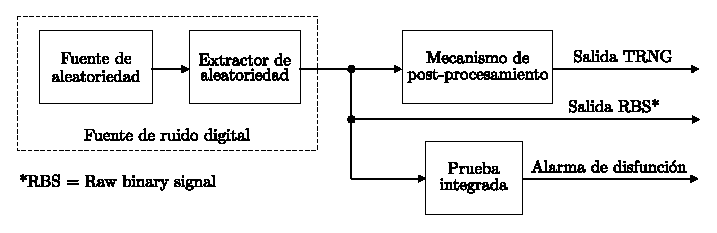
\includegraphics[width=0.9\textwidth]{A0_TRNG_estructura}
            \caption{Estructura general de un TRNG \cite{Badrignans2011}.}
            \label{fig:A1_TRNG_estructura}
        \end{figure}
	
        Los TRNG emplean diferentes fuentes de aleatoriedad y una gran variedad de principios para extraerla. En este sentido, resulta relevante evaluar los principales principios utilizados por los TRNG: parámetros relacionados con la calidad, parámetros relacionados con la seguridad y parámetros relacionados con el diseño.

        \begin{itemize}[noitemsep]
            \item Parámetros relacionados con la calidad
                \begin{itemize}[noitemsep]
                    \item Fuente de aleatoriedad.
                    \item Método de extracción de aleatoriedad y entropía del ruido digital.
                    \item Método de procesamiento posterior aplicado (opcional).
                    \item Tasa de bits de salida y su estabilidad.
                \end{itemize}
            \item Parámetros relacionados con la seguridad
                \begin{itemize}[noitemsep]
                    \item Existencia de un modelo matemático.
                    \item Comprobabilidad interna.
                    \item Seguridad (robustez, resistencia contra ataques).
                \end{itemize}
            \item Parámetros relacionados con el diseño
                \begin{itemize}[noitemsep]
                    \item El uso de recursos.
                    \item El consumo de energía.
                    \item Viabilidad en dispositivos lógicos y FPGAs.
                    \item Automatización del diseño.
                \end{itemize}
        \end{itemize}

        Es fundamental tener en cuenta que no todas las características de los TRNG tienen la misma relevancia en su evaluación. En particular, los parámetros relacionados con la seguridad, tales como la robustez, la disponibilidad de un modelo estocástico y la capacidad de prueba, adquieren una importancia crucial en un sistema de seguridad de datos. Su peso en la evaluación de un TRNG es significativamente mayor que el de otros parámetros, como el consumo de energía o la tasa de bits \cite{Badrignans2011}.

    \section{Condiciones de funcionamiento y calidad de la salida del TRNG}

            Para que un TRNG sea considerado de buena calidad, su salida debe ser prácticamente indistinguible de la salida de un TRNG ideal en todas las condiciones de funcionamiento y a lo largo del tiempo. En el diseño de un TRNG, es fundamental prestar atención tanto a la calidad del flujo de bits generado como a sus parámetros de seguridad, incluyendo la robustez ante el envejecimiento, cambios ambientales, posibles ataques y la existencia de pruebas de autodiagnóstico y en línea \cite{Schindler2003}.
            Un buen TRNG debe proporcionar un flujo de 0s y 1s distribuido uniformemente en su salida. La calidad del flujo de bits generado está estrechamente relacionada con la calidad de la fuente de aleatoriedad y el método utilizado para extraer la aleatoriedad. Las características espectrales de la fuente y el método de extracción determinan los principales parámetros del flujo de bits generado, como el sesgo de los bits de salida, la correlación entre bits sucesivos y patrones visibles. Aunque algunos de estos problemas pueden corregirse mediante un postprocesamiento efectivo, es preferible que el generador produzca intrínsecamente un flujo de bits en bruto de alta calidad.

            Si el extractor muestrea la fuente de aleatoriedad demasiado rápido, los bits adyacentes pueden estar correlacionados. Por esta razón, es una buena práctica comprobar si el flujo de bits generado presenta autocorrelación a corto plazo. Además, pueden existir otras dependencias a corto plazo en el ruido digital, que deben detectarse mediante pruebas específicas del generador. El comportamiento del generador puede verse afectado por interferencias eléctricas externas e internas. Un efecto evidente de estas interferencias son las frecuencias discretas que se originan en la fuente de alimentación y en diversas señales internas que aparecen en el espectro de ruido.

            La señal de ruido generada puede verse significativamente afectada por el ruido de baja frecuencia causado por los semiconductores. Además, las capacidades internas pueden involuntariamente filtrar las frecuencias altas del espectro de ruido. Algunos generadores pueden presentar lo que se conoce como puntos malos, que son breves periodos en los que el generador deja de funcionar debido a interferencias eléctricas o sobrecargas en la parte sobrecargada del circuito.

            Una característica peligrosa del generador es la existencia de una puerta trasera, que se refiere a las desviaciones de la aleatoriedad uniforme introducidas deliberadamente por el fabricante. Por ejemplo, supongamos que en lugar de utilizar un proceso físico, el generador genera una secuencia pseudoaleatoria de alta calidad con una semilla de 40 bits. Aunque sería imposible detectar este comportamiento aplicando pruebas estadísticas estándar al flujo de bits de salida, alguien que conozca la puerta trasera podría adivinar las claves sucesivas mediante un proceso computacionalmente factible. 


    En este trabajo nos enfocaremos en los generadores que pueden implementarse en sistemas digitales y en específico en FPGAs. 

    \section{Trabajos actuales}

        Desde hace una década los TRNGs implementados en FPGA han ido evolucionando y fue en 2016 cuando \cite{Petura2016} hizo una recopilación de todos los núcleos TRNGs que cumplen con las características descritas por la AIS20/31. Los TRNG destinados a ser utilizados en aplicaciones criptográficas deben cumplir con los siguientes requisitos: 1) su diseño debe ser sencillo y comprensible, la fuente de aleatoriedad debe estar claramente definida; 2) el proceso aleatorio subyacente debe ser estacionario y el modelo estocástico debe ser factible; 3) la señal binaria sin procesar debe estar disponible para posteriores pruebas off-line y on-line. Además, es útil que la fuente de aleatoriedad (por ejemplo, el jitter del reloj procedente del ruido térmico) sea cuantificable: su medición dentro del dispositivo puede servir de base para realizar pruebas estadísticas integradas rápidas y eficaces.

        Además seleccionó núcleos TRNG que utilizan circuitos oscilantes: osciladores en anillo de evento único (es decir, osciladores en anillo estándar) \cite{Baudet2010}, \cite{Kohlbrenner2004}, osciladores en anillo multievento con colisiones de señal (es decir, osciladores en anillo de efecto de transición) \cite{Varchola2010}, osciladores en anillo multievento sin colisiones de señal (es decir, anillos autotemporizados) \cite{Cherkaoui2013} y bucles de fase bloqueada (PLL) \cite{Fischer2003}. Todos ellos deberían ser viables en las familias recientes y futuras de FPGAs. Todos ellos utilizan fuentes de aleatoriedad sencillas y comprensibles, su señal aleatoria sin procesar está disponible fuera del generador, y el modelo estocástico del generador existe o es factible. Por lo tanto, todos ellos cumplen los requisitos de AIS-20/31.

    Con base en los criterios del AIS-20/31, los núcleos TRNG adecuados para utilizarse en dispositivos lógicos programables (FPGA) que usan estructuras oscilantes son:

        \begin{itemize}
            \item Elementary ring oscillator based TRNG (ERO-TRNG).
            \item Coherent sampling ring oscillator based TRNG (COSO-TRNG).
            \item Multi-ring oscillator based TRNG (MURO-TRNG).
            \item Transient effect ring oscillator based TRNG (TERO-TRNG).
            \item Self-timed ring based TRNG  (STR-TRNG).
            \item Phase-locked loop based TRNG (PLL-TRNG).
        \end{itemize}

    En años recientes se ha buscado mejorar estos núcleos haciendo variaciones en las conexiones de los componentes internos sin modificar el método de extracción de aleatoriedad. En \cite{Wang2021} se diseño un TRNG basado en PLLs y su contribución se enfocó en analizar su comportamiento a variaciones de voltaje y temperatura, utilizó 56 LUTs, 19 Registros y obtuvo una velocidad de salida de 100 Mbit/s. En \cite{Peetermans2021} se modificó un TRNG basado en el núcleo COSO utilizando una Xilinx Spartan 7, pasó las pruebas estadísticas AIS-31, las NIST y tuvo una velocidad de salida de 1.47 Mbit/s. En \cite{Anandakumar2020} se diseño un TRNG basado en retardos de osciladores de anillo y posteriormente se realizó un postprocesamiento corrector Von Neumann, pasó todas las pruebas NIST, utiliza 528 slices de una Xilinx Spartan 3-A y obtuvo una velocidad de salida de 6 Mbit/s.

    Los artículos anteriores se enfocan en mejorar los núcleos para obtener mejores tasas de bits de salida, disminuir el uso de recursos o mejorar la robustez, sin embargo, existe otro enfoque que consiste en utilizar los TRNG únicamente para generar la semilla de un DRNG. Es decir, crear TRNGs híbridos que combinen las mejores característica de ambos generadores. Además el uso de caos como postprocesamiento o DRNG ha crecido en los años. En \cite{Liao2022} se discretiza un sistema dinámico caótico y se genera una estructura combinada para sembrar el sistema y obtener números aleatorios, se utilizaron 12383 LUTs, 134883 registros, 145 DSPs de una FPGA de la familia Xilinx. En \cite{Vaidyanathan2021} se utiliza un sistema hipercaótico de 5 dimensiones discretizado utilizando los métodos numéricos de forward Euler, trapezoidal, y Runge-Kutta de cuarto orden para diseñar un TRNG híbrido, obtuvo una velocidad de salida de 416 Mbit/s y utiliza 1648 LUTs y 1112 registros. En \cite{Fraga2017} se estudiaron diversos mapas caóticos para utilizarse como DRNG implementados en FPGA, se analizó cual de todos los mapas estudiados genera los mejores resultados y se concluyó que el mapa de corrimientos de Bernoulli es el mejor, utilizando 575 LUTs, 108 registros y obteniendo  una velocidad de salida de 7.389 Mbit/s. En los artículos anteriores se busca aprovechar el caos para aumentar la tasa de bits de salida de los TRNG, sin embargo esto es a costa de aumentar el uso de recursos. 

    Se ha probado extensamente que el caos es una herramienta muy útil para generar números aleatorios y en particular se utiliza mucho para crear esquemas de cifrado \cite{Wong2008,AlHazaimeh2017,Liu2020}, cifrado de imágenes \cite{Li2013, Sivaraman2020,Pareek2006,Kadir2010,Liu2016,Vaidyanathan2018,GarciaGuerrero2020} y en particular los mapas caóticos han cobrado popularidad debido a que su estructura matemática por lo general es sencilla y puede describirse en hardware utilizando pocos recursos, a diferencia de los sistemas dinámicos caóticos en tiempo continuo los cuales requieren el uso de métodos numéricos y su implementación no es trivial.

    Nuevos mapas caóticos \cite{GarciaGrimaldo2021} con mejores características se han estudiado en recientes años lo que abre la posibilidad de poder seguir mejorando los DRNGs. Además sistemas integrados con co-diseño, FPGA-Soc, \cite{HernandezMorales2022} hacen cada vez más fácil poder realizar las pruebas estadísticas en linea y hacer sistemas cada vez más robustos. 

    En este trabajo utilizaremos un TRNG para sembrar un DRNG basado en un mapa caótico bidimensional, probaremos sus características estadísticas utilizando las pruebas NIST y analizaremos la versatilidad del diseño analizando las variaciones del mapa caótico.


    \section{Objetivos}
	
		\subsection{Objetivo general}
			\begin{itemize}
				\item Diseñar e implementar en FPGA un TRNG híbrido para la generación de secuencias muy largas.
			\end{itemize}
		
		\subsection{Objetivos específicos}
			\begin{itemize}
                \item Investigar el estado del arte de diferentes generadores de números aleatorios.
                \item Estudiar los diferentes tipos de generadores de números aleatorios y analizar sus características principales.
                \item Estudiar la teoría de los mapas caóticos y su utilidad en generadores de números aleatorios.
                \item Diseñar un generador de números aleatorios híbrido utilizando un TRNG como generador de semillas y un mapa caótico para realizar un postprocesamiento que mejore sus características estadísticas y comprobar estas utilizando las pruebas NIST.
                \item Implementar el TRNG híbrido en una FPGA.
                %\item Utilizar las pruebas NIST para comprobar sus característica estadísticas.
			\end{itemize}

	\chapter{Selección y evaluación de núcleos TRNGs}		
	
	\section{Variación del reloj (Clock jitter)}
	
	Se supone que una señal de reloj ideal en los dispositivos lógicos digitales es una señal rectangular con un ciclo de trabajo del 50\% y un periodo estable. Pero debido a los diversos ruidos que afectan a los dispositivos electrónicos, la señal de reloj nunca es absolutamente estable y sus flancos se mueven de su posición estable. En otras palabras, la fase de la señal de reloj fluctúa. Esta fluctuación puede verse como una variación del reloj en el dominio del tiempo y como un ruido de fase en el dominio de la frecuencia. En los dispositivos lógicos, una variación del reloj suele ser indeseado, pero inevitable. Dado que estas variaciones afectan negativamente a las comunicaciones de alta frecuencia y a los sistemas de alta velocidad, ha sido bien estudiado y caracterizado.
	
	En los sistemas analógicos, el jitter se caracteriza mejor en el dominio de la frecuencia. De este modo, los componentes de fase y amplitud pueden estudiarse y caracterizarse por separado. En cambio, en los sistemas digitales, las propiedades temporales del jitter son más importantes y, por tanto, el jitter se caracteriza en el dominio del tiempo.
	
	Las variaciones del reloj en un sistema digital es una desviación del flanco de reloj real con respecto a un flanco de reloj ideal. Una señal de reloj ideal se define mediante la ecuación (\ref{eq:periodic}), donde $t(n)$ representa el tiempo del $n$-ésimo periodo de una señal de reloj y $T$ es el periodo de una señal de reloj.
	
	\begin{equation}
		t(n) =  n T
	\label{eq:periodic}
	\end{equation}
	
	Una señal de reloj real no llega siempre a múltiplos enteros de su periodo, como lo hace la ideal, sino que sus flancos fluctúan en torno a este valor a causa del jitter. El jitter está causado por diversos fenómenos físicos, como el ruido térmico, el ruido de la fuente de alimentación, el ruido electromagnético ambiental, etc.	
	
	
	
	\section{Arquitectura de núcleos TRNG seleccionados}

	Con base en los criterios del AIS-20/31, y los núcleos \gls{TRNG} que usan estructuras oscilantes como se clasifican en \cite{Petura2016}:
	
	\begin{itemize}
		\item Single-event ring oscillators
			\begin{itemize}
				\item Elementary ring oscillator based TRNG (\gls{ERO-TRNG})
				\item Coherent sampling ring oscillator based TRNG (\gls{COSO-TRNG})
				\item Multi-ring oscillator based TRNG (\gls{MURO-TRNG})
			\end{itemize}
		\item Multi-event ring oscillators with signal collisions
			\begin{itemize}
				\item Transient effect ring oscillator based TRNG (\gls{TERO-TRNG})
			\end{itemize}
		\item Multi-event ring oscillators without signal collisions
			\begin{itemize}
				\item Self-timed ring based TRNG (\gls{STR-TRNG})
			\end{itemize}
		\item Phase-locked loops
			\begin{itemize}
				\item PLL based TRNG (\gls{PLL-TRNG})
			\end{itemize}
	\end{itemize}
	
		\subsection{Elementary ring oscillator based TRNG (ERO-TRNG)}
		
					
				\begin{figure}[hbtp]
					\caption{Arquitectura del núcleo ERO-TRNG.}
					\centering
					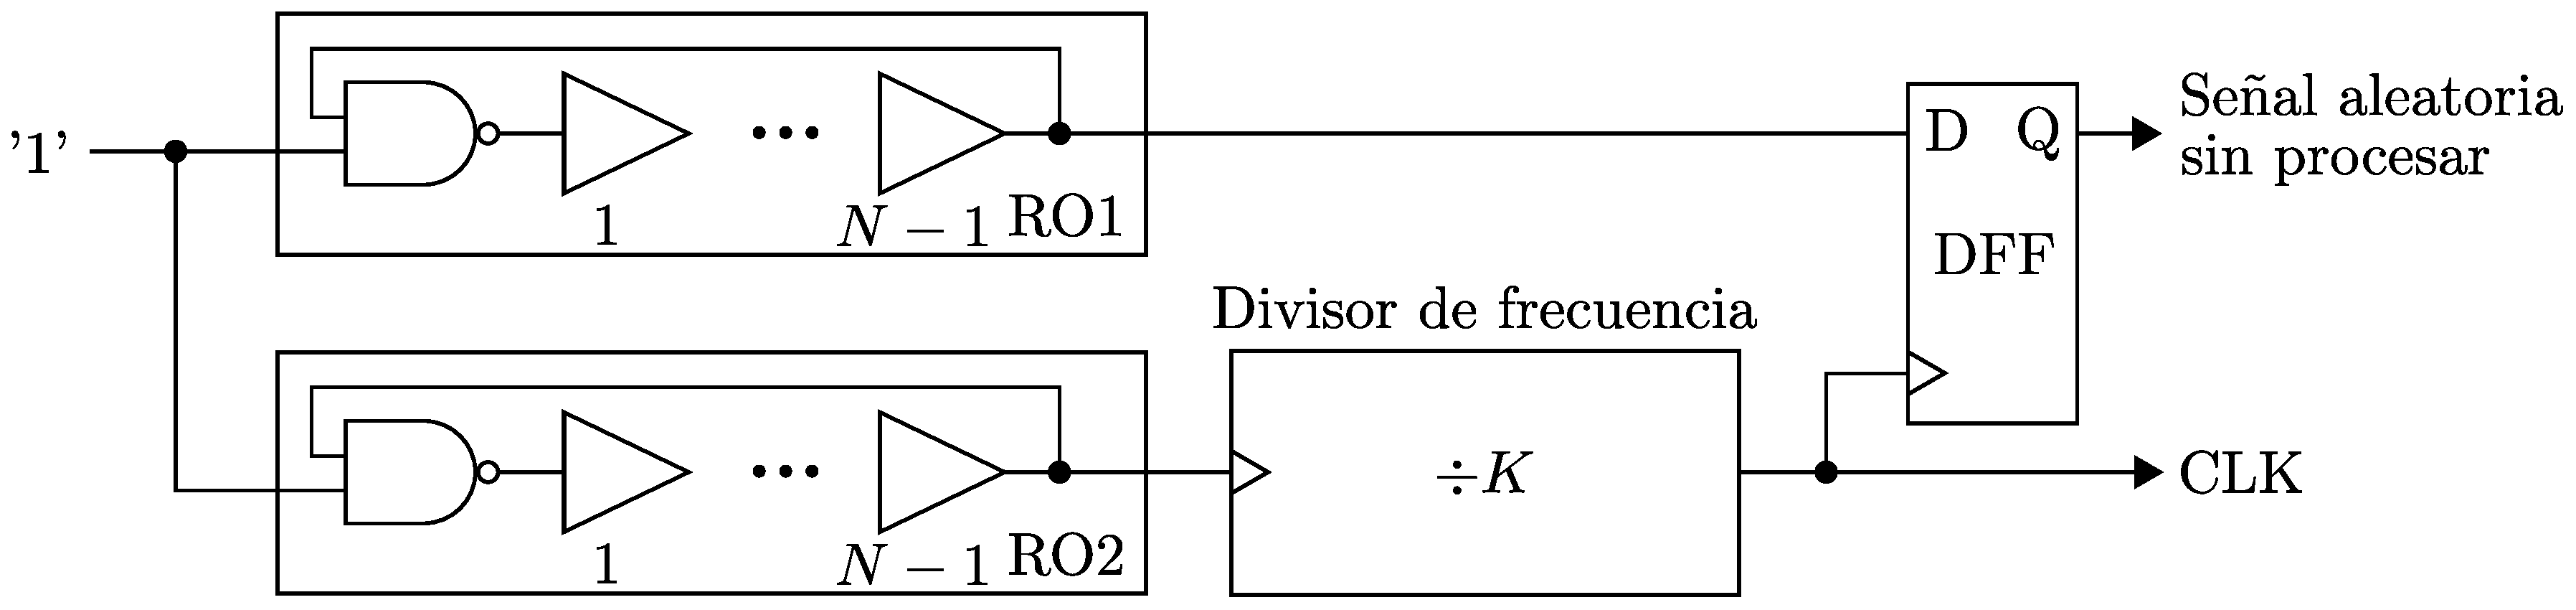
\includegraphics[width=0.8\linewidth]{A1_ERO_TRNG}
					\label{fig:A1_ERO_TRNG}
				\end{figure}
			
			
			
		\subsection{Coherent sampling ring oscillator based TRNG (COSO-TRNG)}
	
				
				\begin{figure}[hbtp]
					\caption{Arquitectura del núcleo COSO-TRNG.}
					\centering
					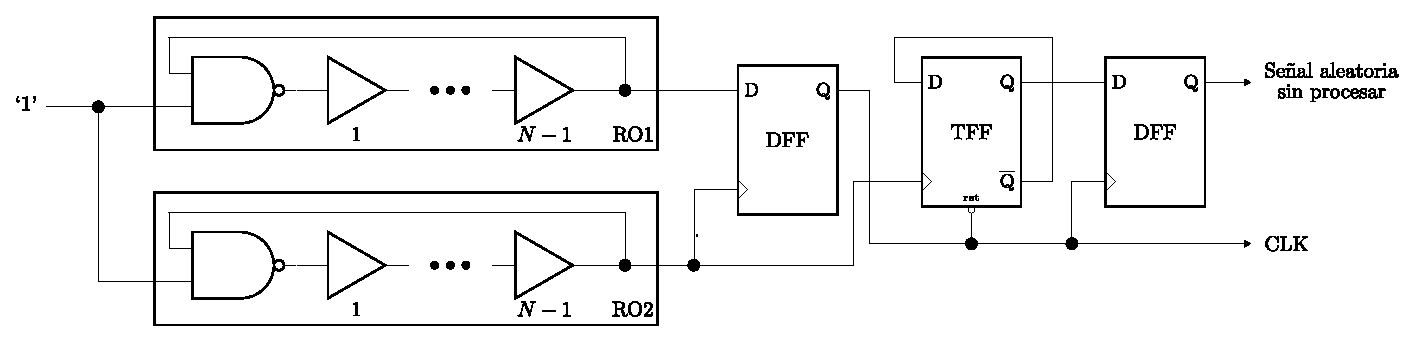
\includegraphics[width=0.8\linewidth]{A2_COSO_TRNG}
					\label{fig:A2_COSO_TRNG}
				\end{figure}
				
				
				
		\subsection{Multi-ring oscillator based TRNG (MURO-TRNG)}
	
				
				\begin{figure}[hbtp]
					\caption{Arquitectura del núcleo MURO-TRNG.}
					\centering
					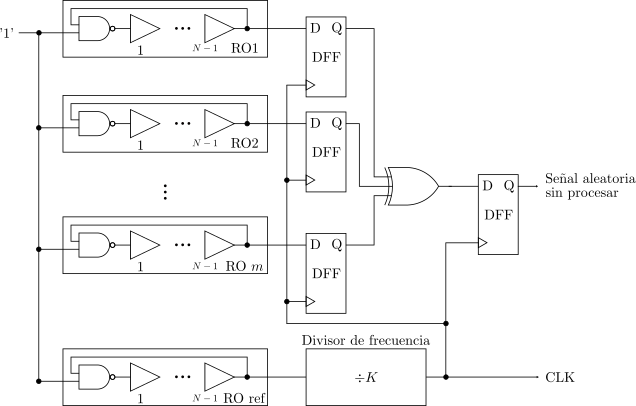
\includegraphics[width=0.8\linewidth]{A3_MURO_TRNG}
					\label{fig:A3_MURO_TRNG}
				\end{figure}
				
				
				
		\subsection{Transient effect ring oscillator based TRNG (TERO-TRNG)}
	
				
				\begin{figure}[hbtp]
					\caption{Arquitectura del núcleo TERO-TRNG.}
					\centering
					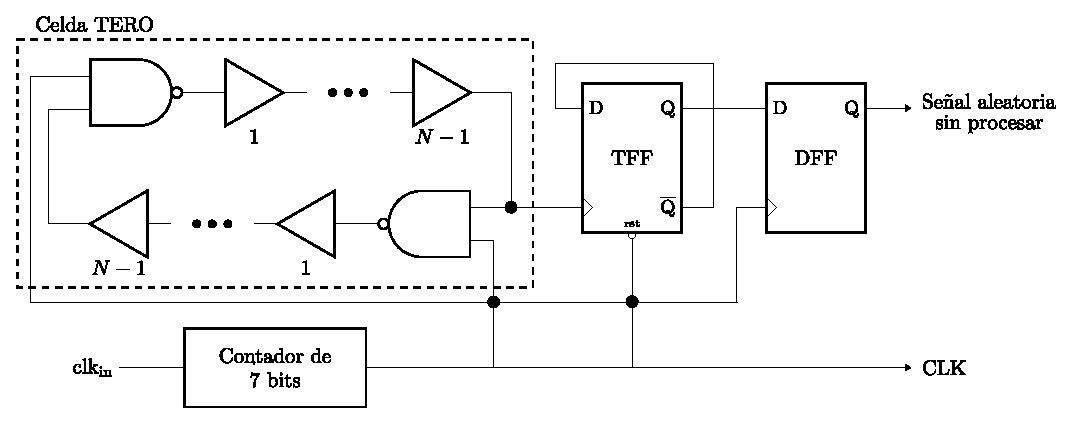
\includegraphics[width=0.8\linewidth]{A4_TERO_TRNG}
					\label{fig:A4_TERO_TRNG}
				\end{figure}
				
				
				
		\subsection{Self-timed ring based TRNG (STR-TRNG)}
	
				
				\begin{figure}[hbtp]
					\caption{Arquitectura del núcleo STR-TRNG.}
					\centering
					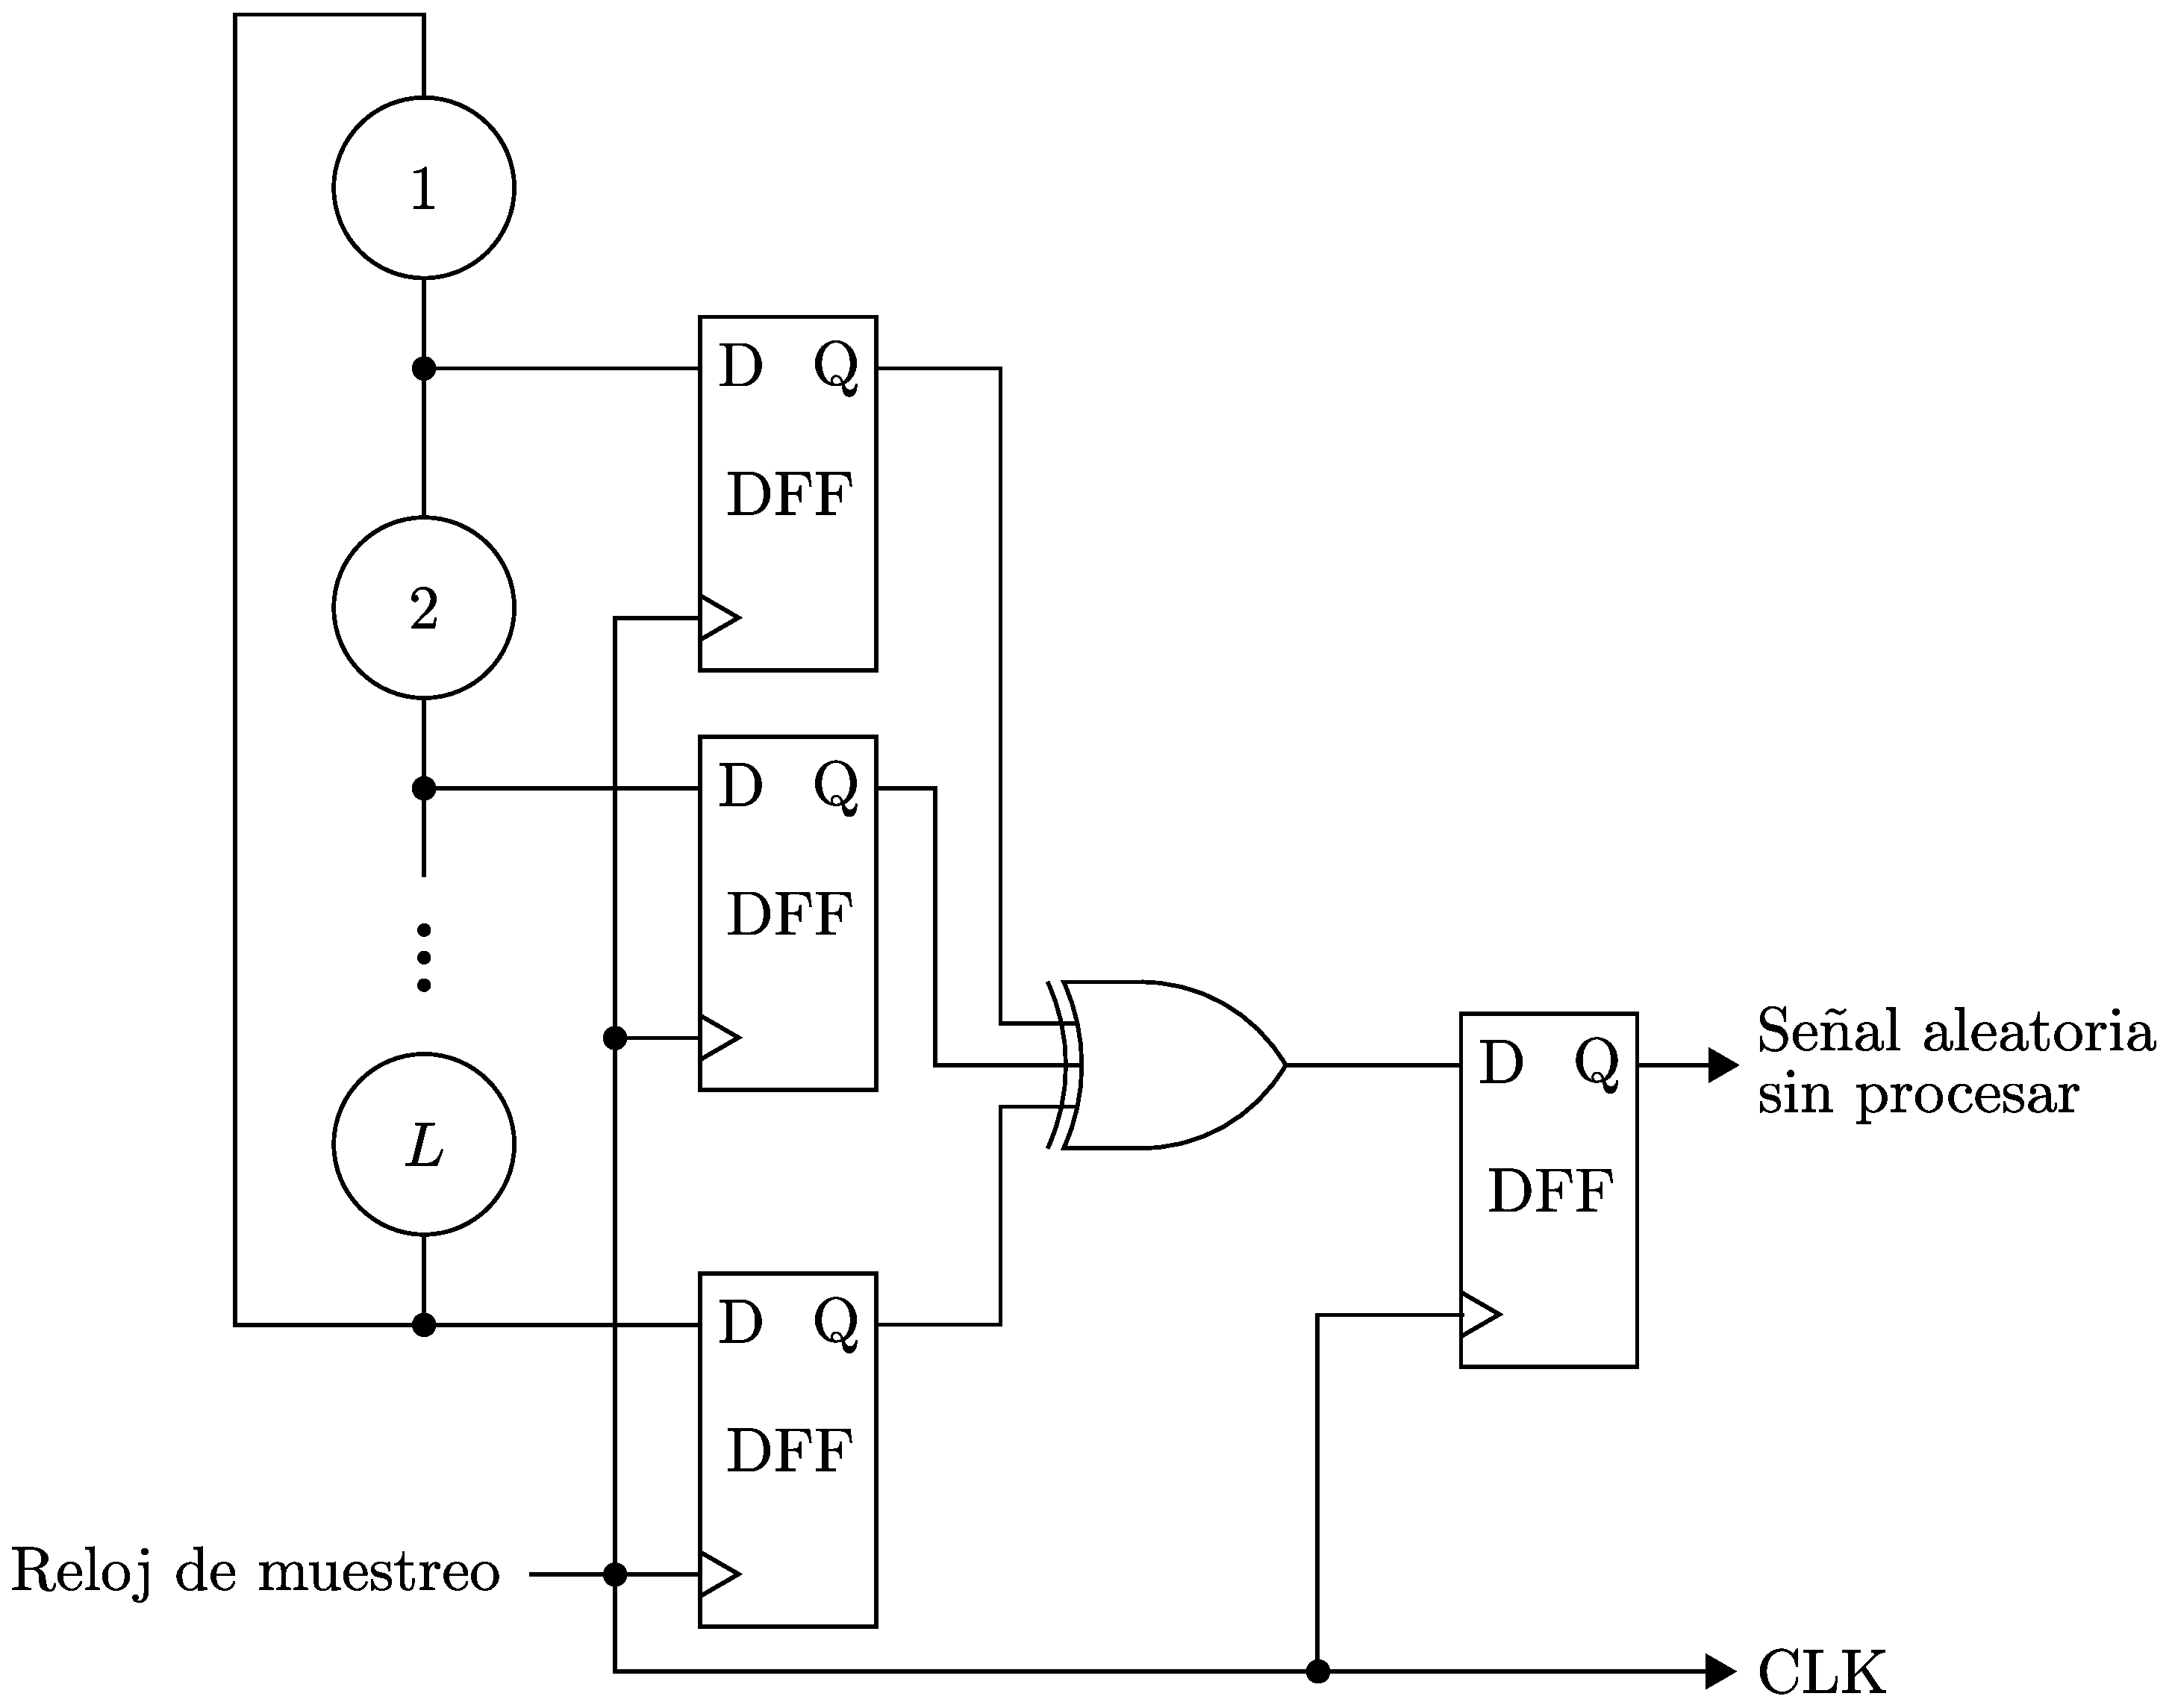
\includegraphics[width=0.8\linewidth]{A5_STR_TRNG}
					\label{fig:A5_STR_TRNG}
				\end{figure}
				
				
				
		\subsection{PLL based TRNG (PLL-TRNG)}
	
				
				\begin{figure}[hbtp]
					\caption{Arquitectura del núcleo PLL-TRNG.}
					\centering
					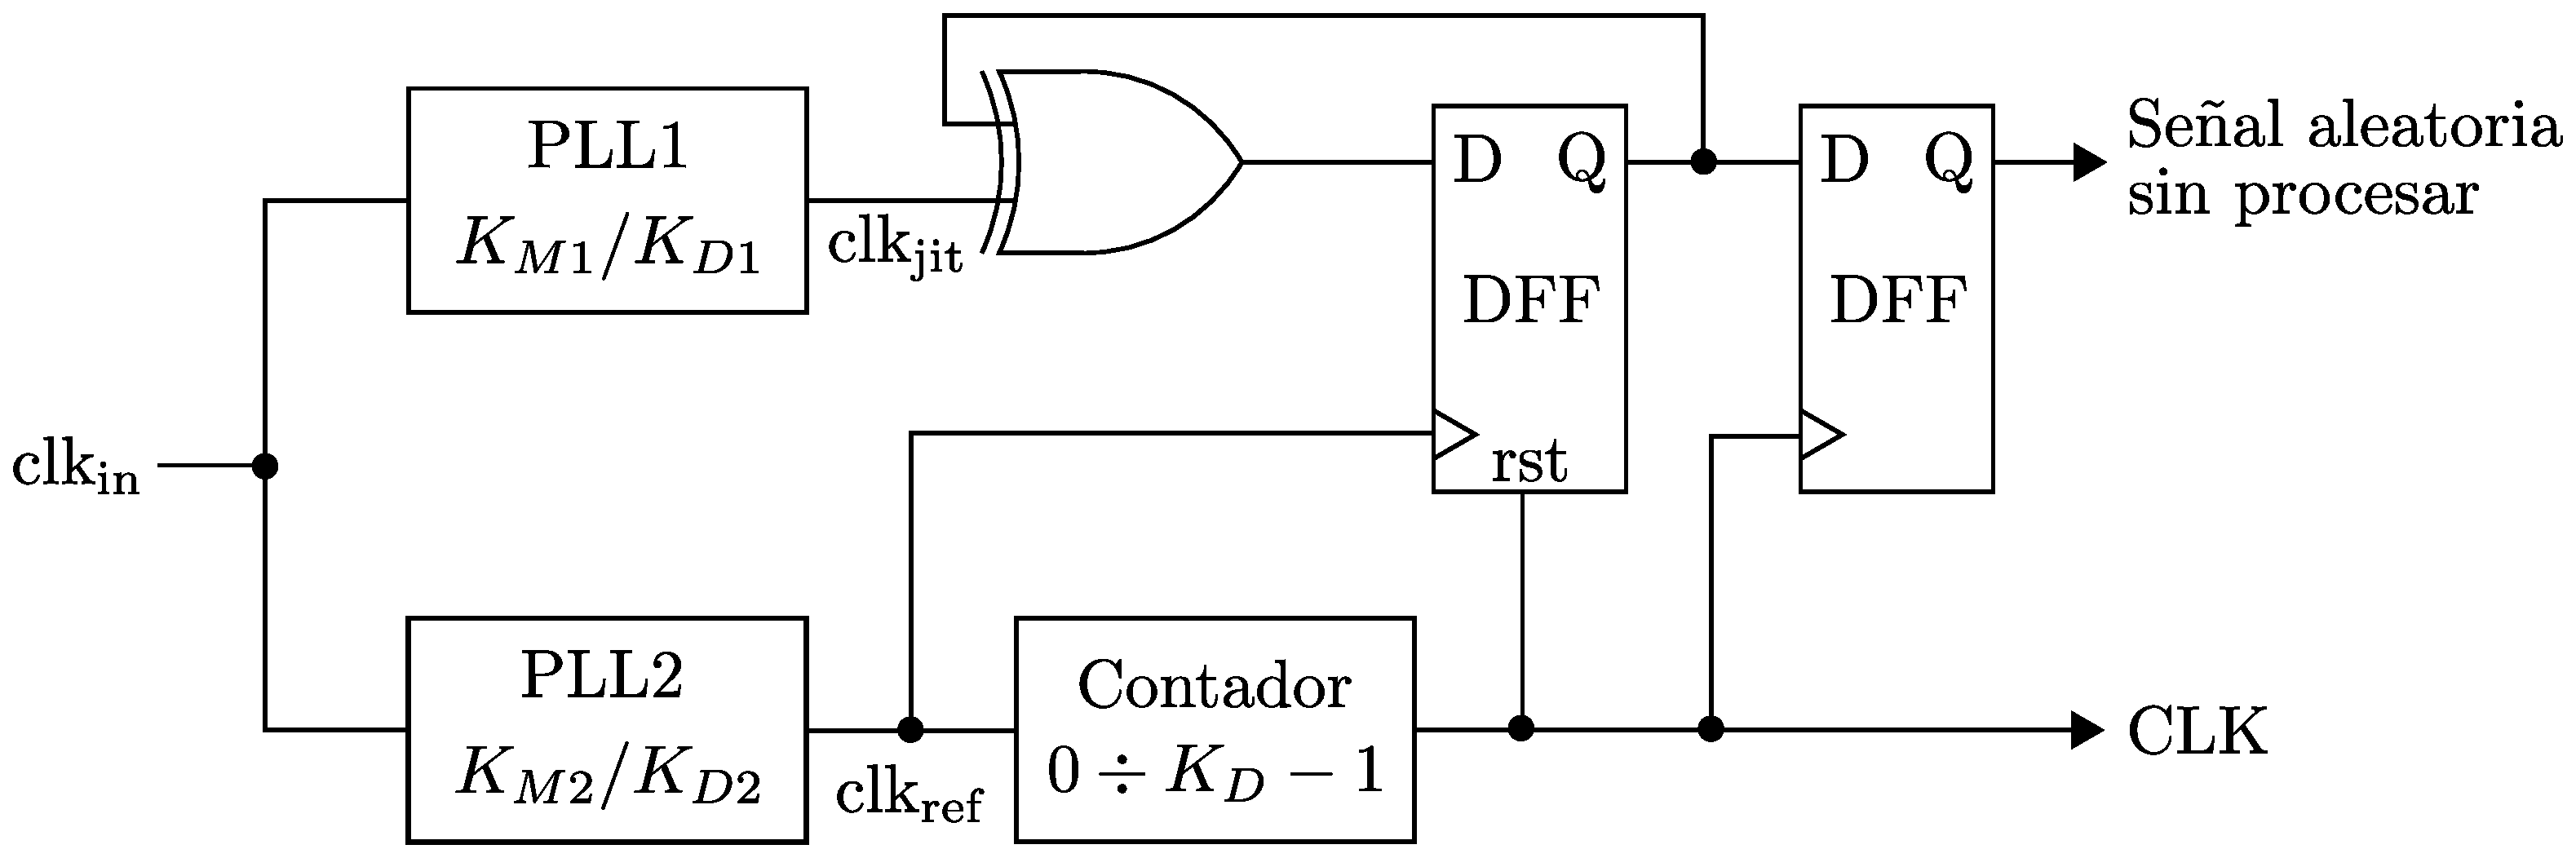
\includegraphics[width=0.8\linewidth]{A6_PLL_TRNG}
					\label{fig:A6_PLL_TRNG}
				\end{figure}
				
				
			
		   



% Table generated by Excel2LaTeX from sheet 'Sheet1'
\begin{table}[htbp]
  \centering
  \caption{Resumen de los resultados de implementación de las TRNGs}
\resizebox{0.8\linewidth}{!}{ 
    \begin{tabular}{|c|c|c|c|c|c|c|c|c|}
    \hline
    \rowcolor[rgb]{ .682,  .667,  .667} TRNG Type & FPGA  & Area  & Power cons. & Bit Rate & Efficiency & Entropy & Entropy * Bit rate & Feasib. \\
    \rowcolor[rgb]{ .682,  .667,  .667}       & device & (LUT/Reg) & [mW]  & [Mbits/s] & [bits/$\mu$Ws] & per bit &       & \& Repeat. \\
    \hline
    \multirow{3}[2]{*}{ERO} & Spartan 6 & 46/19 & 2.16  & 0.0042 & 1.94  & 0.999 & 0.004 & \multirow{3}[2]{*}{5} \\
          & Cyclone V & 34/20 & 3.24  & 0.0027 & 0.83  & 0.990 & 0.003 &  \\
          & SmartFusion 2 & 45/19 & 4     & 0.014 & 3.5   & 0.980 & 0.013 &  \\
    \hline
    \multirow{3}[2]{*}{COSO} & Spartan 6 & 18/3  & 1.22  & 0.54  & 442.6 & 0.999 & 0.539 & \multirow{3}[2]{*}{1} \\
          & Cyclone V & 13/3  & 0.9   & 1.44  & 1600  & 0.999 & 1.438 &  \\
          & SmartFusion 2 & 23/3  & 1.94  & 0.328 & 169   & 0.999 & 0.327 &  \\
    \hline
    \multirow{3}[2]{*}{MURO} & Spartan 6 & 521/131 & 54.72 & 2.57  & 46.9  & 0.999 & 2.567 & \multirow{3}[2]{*}{4} \\
          & Cyclone V & 525/130 & 34.93 & 2.2   & 62.9  & 0.999 & 2.197 &  \\
          & SmartFusion 2 & 545/130 & 66.41 & 3.62  & 54.5  & 0.999 & 3.616 &  \\
    \hline
    \multirow{3}[2]{*}{PLL} & Spartan 6 & 34/14 & 10.6  & 0.44  & 41.5  & 0.981 & 0.431 & \multirow{3}[2]{*}{3} \\
          & Cyclone V & 24/14 & 23    & 0.6   & 43.4  & 0.986 & 0.592 &  \\
          & SmartFusion 2 & 30/15 & 19.7  & 0.37  & 18.7  & 0.921 & 0.340 &  \\
    \hline
    \multirow{3}[2]{*}{TERO} & Spartan 6 & 39/12 & 3.312 & 0.625 & 188.7 & 0.999 & 0.624 & \multirow{3}[2]{*}{1} \\
          & Cyclone V & 46/12 & 9.36  & 1     & 106.8 & 0.987 & 0.985 &  \\
          & SmartFusion 2 & 46/12 & 1.23  & 1     & 813   & 0.999 & 0.999 &  \\
    \hline
    \multirow{3}[2]{*}{STR} & Spartan 6 & 346/256 & 65.9  & 154   & 2343.2 & 0.998 & 154.121 & \multirow{3}[2]{*}{2} \\
          & Cyclone V & 352/256 & 49.4  & 245   & 4959.1 & 0.999 & 244.755 &  \\
          & SmartFusion 2 & 350/256 & 82.52 & 188   & 2286.7 & 0.999 & 188.522 &  \\
    \hline
    \end{tabular}%
}
  \label{tab:addlabel}%

\end{table}%


\gls{FPGA}.

\gls{RNG}.


\gls{TERO}.


	 
	
	
	

	\chapter{Mapas caóticos}

    \section{Definición de caos}
    
    Una manera sencilla de definir el caos sin la necesidad de introducir conceptos muy complicados es como un comportamiento aperiódico, aparentemente impredecible, en sistemas deterministas los cuales presentan extrema sensibilidad a las condiciones iniciales, el más mínimo cambio en la condición inicial produce un resultado muy diferente. \cite{Strogatz1994}

    Según \cite{Sprott2003} los sistemas caóticos tienen las siguientes características:

    \begin{enumerate}
        \item Son aperiódicos, nunca se repiten.
        \item Presentan una dependencia sensible de las condiciones iniciales (y, por tanto, son imprevisibles a largo plazo).
        \item Se rigen por uno o varios parámetros de control, una pequeña modificación de los cuales puede hacer aparecer o desaparecer el caos.
        \item Sus ecuaciones son no lineales.
    \end{enumerate}

    \section{Mapa logístico}

        Cuando nos encontramos con un fenómeno complejo como el caos, que se manifiesta en diversas situaciones, es útil adoptar un enfoque que permita identificar y estudiar el sistema más simple que lo ejemplifica. En este sentido, el mapa logístico representa el sistema matemático caótico más sencillo, ya que utiliza únicamente una variable y un parámetro de control. Las soluciones exactas de este sistema pueden obtenerse mediante álgebra y su representación gráfica facilita su visualización. Este modelo presenta muchas similitudes con sistemas caóticos más complejos, lo que lo convierte en un candidato perfecto para su estudio. De hecho, ha sido utilizado para modelar fenómenos en diversos campos como la ecología, oncología y finanzas.\cite{Sprott2003}

        La ecuación que define al mapa logístico se puede formular partiendo del modelo de crecimiento exponencial en tiempo discreto que se muestra en la ecuación (\ref{eq:crecimiento_exponencial}), donde $A$ es la tasa de crecimiento.

        \begin{equation}
            x_{n+1} = A x_{n}
            \label{eq:crecimiento_exponencial}
        \end{equation}

        Esta ecuación es un ejemplo de un sistema dinámico deterministas, en el que el valor siguiente de $x$ depende únicamente del valor actual. Se trata de un sistema lineal, ya que su representación gráfica muestra una línea recta al graficar $x_{n+1}$ contra $x_{n}$. Se trata de una relación recursiva, ya que se aplica de forma repetida a valores sucesivos de $n$. Además es un ejemplo de mapa iterado, iterar significa retroalimentar la salida de la ecuación a la entrada en el siguiente paso temporal mientas que la iteración es el valor resultante. El término mapa deriva del proceso de transferir cada punto de la Tierra a su correspondiente punto en un mapa impreso. En este caso, estamos mapeando un punto a lo largo del eje $x$ en otro punto a lo largo del mismo eje como se muestra en la Figura \ref{fig:F0_mapdiagram}. Sin embargo para mapas más complicados el mapeo se puede extender a más de una dimensión. A la secuencia $x_{0}, x_{1}, x_{2} , \ldots $ es la órbita del mapa comenzando desde $x_{0}$.

        \begin{figure}[hbtp]
            \caption{Ejemplo de mapeo en una dimensión.}
            \centering
            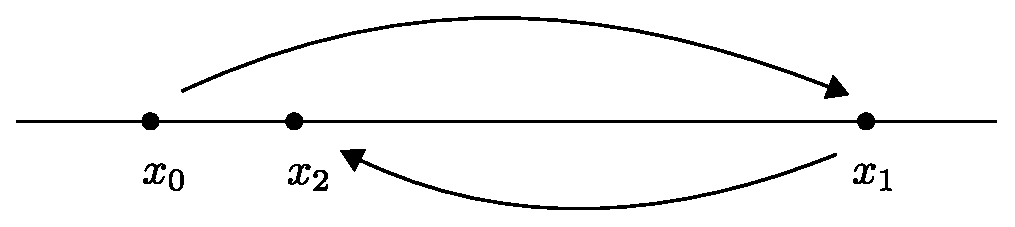
\includegraphics[width=0.7\textwidth]{F0_mapdiagram}
            \label{fig:F0_mapdiagram}
        \end{figure}

        Si el parámetro $A > 1$ el sistema presenta un crecimiento exponencial mientras que si $0 < A < 1$ presenta un decaimiento exponencial. Para toda condición inicial $x_{0}$ el sistema es atraído al punto $x = 0$ si $0 < A < 1$ y es atraído hacia el infinito si $A > 1$. Los sistemas cuya solución es atraída hacia el infinito son conocidos no acotado. El termino $A$ es un parámetro de control que rige la naturaleza de la dinámica. El valor $A = 1$ separa dos regiones en las que el comportamiento difiere y se denomina punto de bifurcación. Si $|A| < 1$ el sistema oscila alrededor de $x = 0$ y su amplitud decrece con el tiempo. Por lo tanto $x = 0$ es un atractor para toda $x_{0}$ cuando $|A| < 1$. Sin embargo cuando $A< -1$ crece exponencialmente hacia el infinito.

        Como el crecimiento exponencial no puede continuar para siempre, la ecuación (\ref{eq:crecimiento_exponencial}) es poco realista para cualquier proceso natural. Típicamente, alguna no linealidad detiene e incluso revierte el crecimiento. La no linealidad es despreciable en pequeños valores de $x$ pero empieza a dominar mientras más crece $x$. Una estrategia comúnmente utilizada es analizar primero el comportamiento lineal antes de introducir no linealidades. A pesar de que el sistema lineal pueda presentar deficiencias notorias, es importante comprender sus propiedades. 

        Imaginemos un cultivo de bacterias que crece cada hora, con las condiciones ideales de crecimiento la población aumenta sin restricciones y podemos modelar este comportamiento con la ecuación (\ref{eq:crecimiento_exponencial}). No obstante, si el espacio o el alimento escasea la población de bacterias no puede continuar creciendo a este ritmo. A medida que aumenta la población, el alimento y algunas bacterias mueren antes de poder dividirse. 

        Para incluir un término que reduzca el crecimiento a medida que $x$ aumenta es necesario modificar la ecuación (\ref{eq:crecimiento_exponencial}). La manera más sencilla es considerado que la tasa de crecimiento decrece linealmente, de manera que a la ecuación (\ref{eq:ecuacion_logistica}) se le conoce como ecuación logística.
            
       \begin{equation}
            x_{n+1} = A x_{n} (1 - x_{n}) 
            \label{eq:ecuacion_logistica}
       \end{equation}

       La no linealidad es cuadrática, debido a que el modelo se puede reescribir como $x_{n+1} = A x_{n} - A x_{n}^{2}$. El término cuadrático da una retroalimentación negativa no lineal y limita el crecimiento. La Figura \ref{fig:F1_logistic_curve} muestra la gráfica de la ecuación (\ref{eq:ecuacion_logistica}) con $A = 4$ llamada función logística o curva logística, la cual es una parábola.


        \begin{figure}[hbtp]
            \caption{El mapa logístico con $A = 4$.}
            \centering
            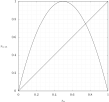
\includegraphics[width=0.6\textwidth]{F1_logistic_curve}
            \label{fig:F1_logistic_curve}
        \end{figure}

        En la Figura \ref{fig:F0_mapdiagram} también se muestra una recta descrita por $x_{n+1} = x_{n}$, a $45^{\circ}$ cuyas intersecciones con la parábola dan los valores de $x$ que no cambian con el tiempo. Para un mapa cuadrático, hay dos intersecciones de este tipo, que corresponden a las soluciones de la ecuación cuadrática que resultan de establecer $x_{n+1} = x_{n} = x^{*}$. Las soluciones $x^{*} = 0$ y $x^{*} = 1 - 1/A$ son llamados puntos fijos del mapa.

        Es interesante examinar cómo $x$ se aproxima a un punto fijo partiendo de una condición inicial $x_{o} \neq x^{*}$, esto lo hacemos con un diagrama de cobwebs. Los diagramas de cobwebs son una herramienta valiosa que nos permiten observar el comportamiento global de un sistema de manera intuitiva, proporcionando información complementaria a la obtenida mediante el análisis lineal. Son especialmente útiles resultan cuando el análisis lineal no es suficiente.

        Para construir el diagrama de cobwebs de un mapa iterado realizamos los siguientes pasos:

        Dado $x_{n+1} = f(x_{n})$ y una condición inicial $x_{0}$, trazar una línea vertical hasta que intersecte la gráfica $f$, esa altura es la salida $x_{1}$, en otras palabras dibujar una línea vertical desde $(x_{0}, 0) $ hasta $(x_{0}, x_{1})$. Después trazar una horizontal hasta intersectar con la linea diagonal $x_{n+1} = x_{n}$, es decir, dibujar una línea desde  $(x_{0}, x_{1}) $ hasta $(x_{1}, x_{1})$. Después trazar otra línea vertical hasta que intersecte la gráfica $f$ otra vez, una línea desde $(x_{1}, x_{1}) $ hasta $(x_{1}, x_{2})$. Repetir este proceso $n$ veces para generar los primeros $n$ puntos en la órbita.

        \begin{figure}[hbtp]
            \caption{Diagrama de cobwebs de mapa logístico con $A = 2.8$ y $x_{0} = 0.2$.}
            \centering
            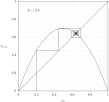
\includegraphics[width=0.6\textwidth]{F2_cobwebs_simple}
            \label{fig:F2_cobwebs_simple}
        \end{figure}

        Para el mapa logístico con $1 < A < 3,$ todos los puntos inicales en el intervalo $0 < x_{0} < 1$ se aproximan al punto fijo $x^{*} = 1 - 1/ A $, aunque la solución puede oscilar a su alrededor antes de llegar al valor final. El comportamiento recuerda al de un péndulo simple que oscila alrededor de la vertical antes de que la fricción lo lleve a reposar en su posición final. Otra manera de visualizar este comportamiento es gráficas la serie de tiempo, $x_{n}$ contra $n$, como se ve en la Figura \ref{fig:F3_time_series}. Es importante hacer la aclaración que se dibujaron lineas entre cada iteración para una mejor visualización, pero los datos son discretos. 

        \begin{figure}[hbtp]
            \caption{Serie de tiempo de mapa logístico con $A = 2.8$.}
            \centering
            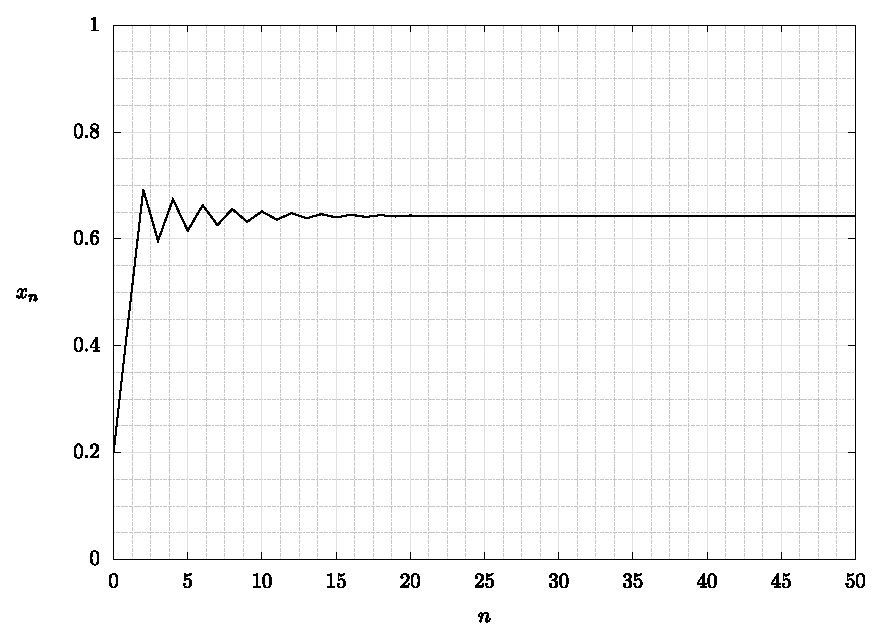
\includegraphics[width=0.6\textwidth]{F3_time_series}
            \label{fig:F3_time_series}
        \end{figure}

        En la ecuación de crecimiento exponencial en tiempo discreto (\ref{eq:crecimiento_exponencial}) cuando $A = \pm 1$ el comportamiento cambia abruptamente de acotado a no acotado. La ecuación logística se comporta de manera simular, excepto que hay más bifurcaciones y el comportamiento en varias regiones es más diverso e interesante. Es útil estudiar las bifurcaciones del mapa logístico porque las características generales son comunes a muchos sistemas caóticos. Consideraremos sólo valores positivos de $A$ y $x$.

        \begin{itemize}
            \item Caso $0 < A < 1$.
                En este rango la parábola solo puede intersectar a la linea de $45^{\circ}$ una vez en valores no negativos, y por lo tanto solo hay un punto fijo en $x^{*} = 0$. Todas las condiciones iniciales en el rango $0 < x_{o} < 1$ son atraídos hacia el punto $x^{*} = 0$. Decimos que estos puntos se encuentran dentro de una cuenca de atracción de $x_{0}$ y que el punto fijo $x_{0}$ es estable. Todos los puntos dentro de la cuenca de atracción se acercan al punto fijo con cada iteración. La no linealidad tiene poco efecto después de las primeras iteraciones. Los valores de $x_{0}$ fuera de de la cuenca de atracción están no acotados, escapan al infinito.
            \item Caso $1 < A < 3$.
                Al igual que con la ecuación (\ref{eq:crecimiento_exponencial}), para A = 1 se produce una bifurcación y el punto fijo en $x^{*} = 0$ se vuelve inestable. El atractor se convierte en un repulsor. Si $x$ resulta ser exactamente cero, permanecerá así, pero si es incluso ligeramente positivo, crecerá inicialmente a un ritmo exponencial. La situación es como la de un lápiz apoyado sobre su extremo puntiagudo. El más mínimo empujón hará que se caiga. Sin embargo, a diferencia de la ecuación (\ref{eq:crecimiento_exponencial}) en la que las soluciones son ilimitadas, el mapa logístico en $A = 1 $ desarrolla un nuevo punto fijo en $x^{*} = 1- 1/A = 0$ que se aleja de cero para $A > 1$. Si $A$ no es demasiado grande, entonces ese punto es un atractor porque todos los valores iniciales en el rango $0 < x_{0} < 1$ son atraídos hacia él y finalmente se asientan en él. Decimos que el estado final es un ciclo de periodo 1, o simplemente un ciclo de 1, porque cada iteración es la misma que la anterior. Si la ecuación logística estuviera modelando la población de bacterias, entonces predeciría un crecimiento exponencial inicial para este rango de $A$, pero un estado estacionario final en el que el número de bacterias no cambia.
            \item Caso $3 < A < 3.44948$.
                Para $A = 3$, el punto fijo en $x^{*} = 1 - 1/A$ sigue existiendo, pero cambia de estable a inestable, convirtiéndose en un repulsor. Esta bifurcación se produce cuando la pendiente de la parábola en el punto fijo es igual a $-1$. Para $A > 3$ tenemos un crecimiento exponencial alejándonos del punto, en lugar de una caída exponencial hacia él. Como la pendiente es negativa, la solución oscila a ambos lados del punto fijo mientras se aleja, igual que en la ecuación (\ref{eq:crecimiento_exponencial}) con $ A < -1$. De ahí que la bifurcación en $A = 3$ se denomine flip. Sin embargo, el crecimiento no continúa para siempre. En su lugar, se acerca a una condición en la que cada iterado es el mismo $x_{n} = x_{n+2} = x_{n+4}$ como en el diagrama de cobwebs de la Figura \ref{fig:F5_cobwebs_bifurcation} Con un poco de álgebra, esta condición puede reducirse a una ecuación de cuarto grado.

                \begin{equation}
                    A^{3} x^{4} - 2 A^{3} x^{3} + A^{2} (A + 1) x^{2} - (A^{2} -1)x = 0
                \end{equation}

                Como cualquier ecuación cuadrática, tiene cuatro raíces. 


                


        \begin{figure}[hbtp]
            \caption{Diagrama de cobwebs de mapa logístico con $A = 3.2$ y $x_{0} = 0.1$.}
            \centering
            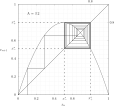
\includegraphics[width=0.6\textwidth]{F5_cobwebs_bifurcation}
            \label{fig:F5_cobwebs_bifurcation}
        \end{figure}


        \begin{figure}[hbtp]
            \caption{Diagrama de bifurcación de mapa logístico.}
            \centering
            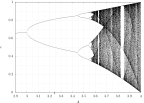
\includegraphics[width=0.6\textwidth]{F4_bifurcation}
            \label{fig:F4_bifurcation}
        \end{figure}


        \end{itemize}

    \section{Análisis de mapa logístico}

        Consideremos la ecuación $x_{n+1} = A x_{n} (1 - x_{n})$ para $0 \leq x_{n} \leq 1$ y $0 \leq A \leq 4$. Los puntos fijos satisfacen $x^{*} = f(x^{*}) = A x^{*}(1 - x^{*})$. Por lo tanto $x^{*} = 0$  o $x^{*} = 1 - 1/A$. El origen es un punto fijo para todas las $A$, mientras que $x^{*} = 1 - 1/A$ solo es valido para las $x \geq 1$. La estabilidad depende de $f'(x^{*}) = A - 2Ax^{*}$. Como $f'(0) = A $ el origen es estable para $A < 1$ e inestable para $A < 1$. En el otro punto fijo, $f'(x^{*}) = A - 2 A \left( 1 - \frac{1}{A} \right) = 2 - A$. Entonces $x^{*} 1 - \frac{1}{A} $ es estable para $1 < A < 3$.

    \section{Puntos fijos y estabilidad lineal}
        

            

Libro para el publico general \cite{Gleick1987}
 

	\chapter{Implementación}

	\section{Mapa caótico}
    
        En el artículo \cite{Sprott1993} y \cite{Fraga2021}
        \begin{equation}
            \begin{array}{ccl}
                x_{n+1} & = &  a_{1} + a_{2}x_{n} + a_{3}x_{n}^{2} + a_{4}x_{n}y_{n} + a_{5}y_{n} + a_{6}y_{n}^{2}\\
                y_{n+1} & = &  a_{7} + a_{8}x_{n} + a_{9}x_{n}^{2} + a_{10}x_{n}y_{n} + a_{11}y_{n} + a_{12}y_{n}^{2}
            \end{array}
        \end{equation}
        
        donde los parámetros $\{a_{1}, a_{2}, \ldots a_{12}\}$ pueden tomar diferentes valores, sin embargo para este trabajo se usaron los siguientes:


        \begin{equation}
            \begin{array}{ccl}
                x_{n+1} & = &  a_{1} + ( a_{2} + a_{3}x_{n} )x_{n} + a_{4}x_{n}y_{n} + ( a_{5} + a_{6}y_{n} )y_{n} \\
                y_{n+1} & = &  a_{7} + ( a_{8} + a_{9}x_{n} )x_{n} + a_{10}x_{n}y_{n} + ( a_{11} + a_{12}y_{n})y_{n}
            \end{array}
        \end{equation}

        \begin{equation}
             \begin{array}{lcl}
                M_{1} & = & \{ -0.6, -0.1, 1.1, 0.2, -0.8, 0.6, -0.7, 0.7, 0.7, 0.3, 0.6, 0.9 \}\\
                M_{2} & = & \{ -1.0, 0.9, 0.4, -0.2, -0.6, -0.5, 0.4, 0.7, 0.3, -0.5, 0.7, -0.8 \}\\
                M_{3} & = &  \{0.8, 1.0, -1.2, -1.0, 1.1, -0.9, 0.4, -0.4, -0.6, -0.2, -0.5, -0.7 \}\\
                M_{4} & = & \{-0.6, -0.4, -0.4, -0.8, 0.7, 0.3, -0.4, 0.4, 0.5, 0.5, 0.8, -0.1 \}
            \end{array}
        \end{equation}

        \begin{equation}
            \begin{array}{lcl}
                s_{n+1} = \{ x_{n+1} \text{ mod } 256, y_{n+1} \text{ mod } 256 \}
            \end{array}
        \end{equation}

        \begin{table}[htbp]
            \centering
            \caption{Exponentes de Lyapunov y dimensión fractal (tomados de \cite{Sprott1993}) de los mapas 2D usados.}
            \begin{tabular}{|l|l|l|}
                \hline
                \rowcolor{lightgray} Mapa  & Exponentes de Lyapunov & Dimensión fractal \\
                \hline
                1     & 0.12                   & 1.77   \\
                \hline
                2     & 0.14                   & 1.79   \\
                \hline
                3     & 0.15                   & 1.69   \\
                \hline
                4     & 0.13                   & 1.50   \\
                \hline
            \end{tabular}
        \end{table}

        \begin{table}[htbp]
            \centering
            \caption{Número de bits usados en la implementación de cada uno de los mapas con aritmética de punto fijo.}
            \begin{tabular}{|l|l|l|}
                \hline
                \rowcolor{lightgray} Mapa  & Bits parte entera & Bits parte fraccionaria \\
                \hline
                1     & 3                   & 60   \\
                \hline
                2     & 4                   & 59   \\
                \hline
                3     & 4                   & 59   \\
                \hline
                3     & 3                   & 60   \\
                \hline
            \end{tabular}
        \end{table}

        \begin{table}[htbp]
            \centering
            \caption{Rangos usados para la condición inicial para cada uno de los mapas.}
            \begin{tabular}{|l|l|}
                \hline
                \rowcolor{lightgray} Mapa  & Rango de valores para $x_{0}$ y $y_{0}$ \\
                \hline
                $M_{1}$  & $x_{0} \in [-0.5, \phantom{-} 0.5]$, $y_{0} \in [-0.5, \phantom{-}0.5]$ \\
                \hline
                $M_{2}$  & $x_{0} \in [-1.0, \phantom{-} 0.0]$, $y_{0} \in [\phantom{-}0.0, \phantom{-}1.0]$ \\
                \hline
                $M_{3}$  & $x_{0} \in [\phantom{-}0.0, \phantom{-} 1.0]$, $y_{0} \in [-0.6, \phantom{-}0.4]$ \\
                \hline
                $M_{4}$  & $x_{0} \in [-1.5, -0.5]$, $y_{0} \in [-0.5, \phantom{-}0.5]$ \\
                \hline
            \end{tabular}
        \end{table}

        \begin{figure}[hbtp]
            \caption{Diagrama de bloques del mapa caótico.}
            \centering
            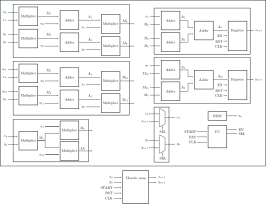
\includegraphics[width=0.9\linewidth]{B1_architecture}
            \label{fig:B1_architecture}
        \end{figure}

        \begin{figure}[hbtp]
            \caption{Máquina de estados de mapa caótico.}
            \centering
            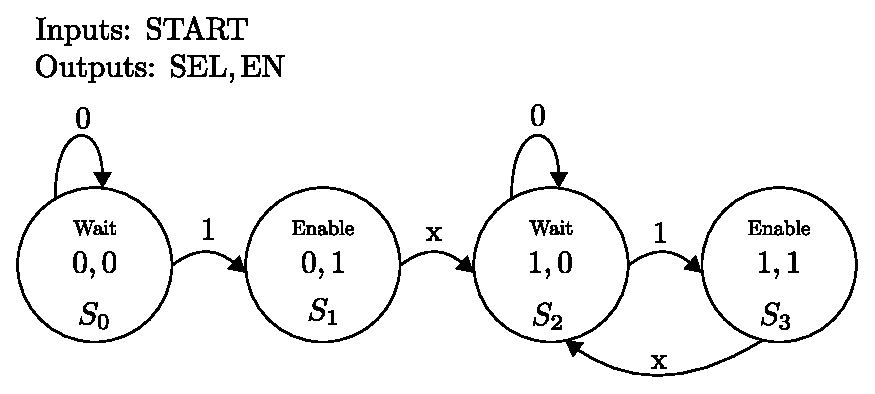
\includegraphics[width=0.6\linewidth]{B2_fsm_cm}
            \label{fig:B2_fsm_cm}
        \end{figure}

        \begin{figure}[hbtp]
            \caption{Simulación del mapa caótico en punto flotante.}
            \centering
            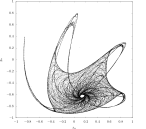
\includegraphics[width=0.8\linewidth]{B0_chaotic_map}
            \label{fig:B0_chaotic_map}
        \end{figure}

    \section{Single Constant Multiplier (SCM)}


    \section{Comunicación RS232}

        \begin{figure}[hbtp]
            \caption{Diagrama de bloques de transmisión RS232.}
            \centering
            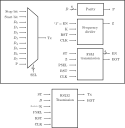
\includegraphics[width=0.6\linewidth]{C1_architecture_rs232}
            \label{fig:C1_architecture_rs232}
        \end{figure}

        \begin{figure}[hbtp]
            \caption{Máquina de estados para la transmisión RS232.}
            \centering
            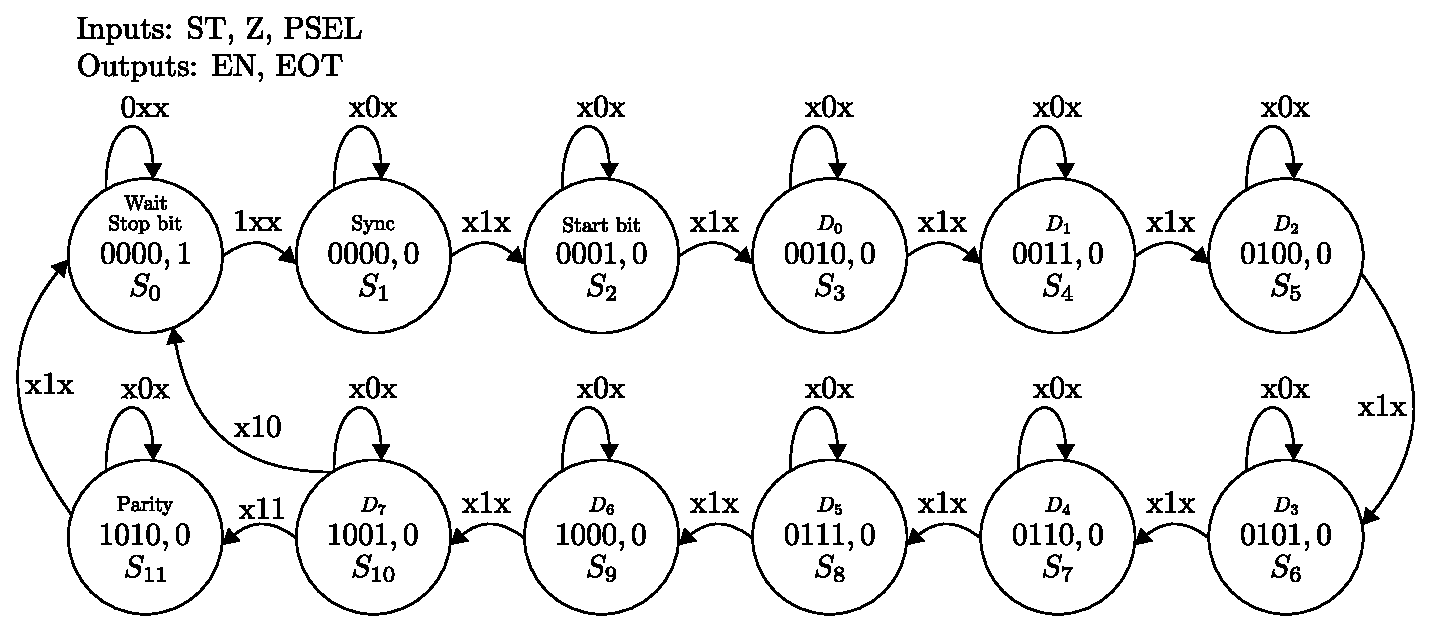
\includegraphics[width=0.8\linewidth]{C0_fsm_rs232}
            \label{fig:C0_fsm_rs232}
        \end{figure}	

    \section{Diseño de TRNG}

        \begin{figure}[hbtp]
            \caption{Diagrama de bloques de TRNG.}
            \centering
            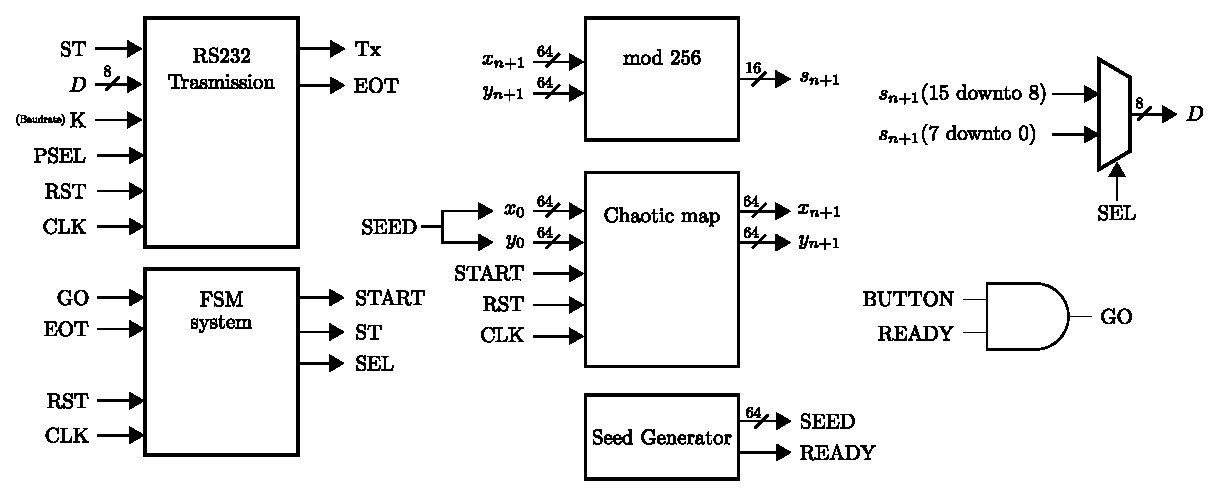
\includegraphics[width=0.9\linewidth]{D0_system}
            \label{fig:D0_system}
        \end{figure}

        \begin{figure}[hbtp]
            \caption{Máquina de estados de TRNG.}
            \centering
            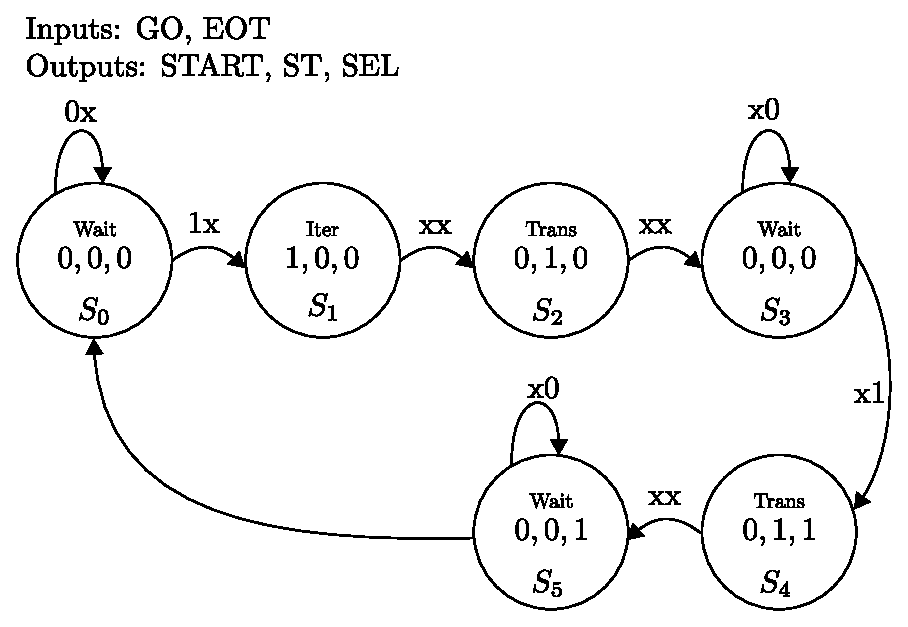
\includegraphics[width=0.7\linewidth]{D1_fsm_system}
            \label{fig:D1_fsm_system}
        \end{figure}

	\begin{comment}

	
\begin{table}[htbp]
  \centering
  \caption{Resumen de los resultados de implementación de las TRNGs}
\resizebox{0.5\linewidth}{!}{ 
    \begin{tabular}{lll}
   & Test name                 & Prop. \\
   \hline
1  & Frequency                 & 0.99  \\
2  & Block frequency           & 0.99  \\
3  & Runs                      & 1.00     \\
4  & Longest run               & 1.0     \\
5  & Rank                      & 0.98  \\
6  & DFT                       & 0.99  \\
7  & Non-overlapping templates & 1.00     \\
8  & Overlapping templates     & 0.99  \\
9  & Universal                 & 0.99  \\
10 & Linear complexity         & 0.99  \\
11 & Serial                    & 0.99  \\
12 & Approximate Entropy       & 0.99  \\
13 & Cumulative Sums           & 0.99  \\
14 & Random excursions         & 0.99  \\
15 & Random excursions variant & 1.00    
    \end{tabular}
}
  \label{tab:asdasd}
\end{table}


\newpage
	




	\end{comment}


	\chapter{Implementación}

	\section{Mapa caótico}
	
	\subsection{Modelo matemático}
	En el artículo \cite{Sprott1993} y \cite{Fraga2021}
	\begin{equation}
	 \begin{array}{ccl}
		x_{n+1} & = &  a_{1} + a_{2}x_{n} + a_{3}x_{n}^{2} + a_{4}x_{n}y_{n} + a_{5}y_{n} + a_{6}y_{n}^{2}\\
		y_{n+1} & = &  a_{7} + a_{8}x_{n} + a_{9}x_{n}^{2} + a_{10}x_{n}y_{n} + a_{11}y_{n} + a_{12}y_{n}^{2}
		\end{array}
	\end{equation}
	
	donde los parámetros $\{a_{1}, a_{2}, \ldots a_{12}\}$ pueden tomar diferentes valores, sin embargo para este trabajo se usaron los siguientes:
	
	
	
	\begin{equation}
	 \begin{array}{ccl}
		x_{n+1} & = &  a_{1} + ( a_{2} + a_{3}x_{n} )x_{n} + a_{4}x_{n}y_{n} + ( a_{5} + a_{6}y_{n} )y_{n} \\
		y_{n+1} & = &  a_{7} + ( a_{8} + a_{9}x_{n} )x_{n} + a_{10}x_{n}y_{n} + ( a_{11} + a_{12}y_{n})y_{n}
		\end{array}
	\end{equation}
	
	
	\begin{figure}[hbtp]
		\caption{Arquitectura a bloques del mapa caótico.}
		\centering
		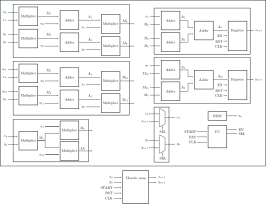
\includegraphics[width=0.9\linewidth]{B1_architecture}
		\label{fig:B1_architecture}
	\end{figure}
	
	
	\begin{figure}[hbtp]
		\caption{Máquina de estados de mapa caótico.}
		\centering
		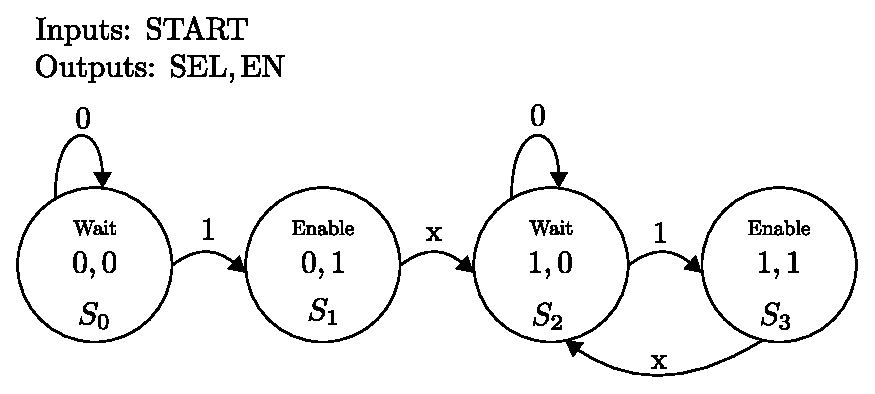
\includegraphics[width=0.6\linewidth]{B2_fsm_cm}
		\label{fig:B2_fsm_cm}
	\end{figure}
	
	
	Simulación del sistema en punto flotante en C
	
	\begin{figure}[hbtp]
		\caption{Mapa caótico.}
		\centering
		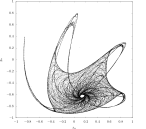
\includegraphics[width=0.8\linewidth]{B0_chaotic_map}
		\label{fig:B0_chaotic_map}
	\end{figure}
	
	
	
	\section{Comunicación RS232}
	
	\begin{figure}[hbtp]
		\caption{Máquina de estados para transmisión.}
		\centering
		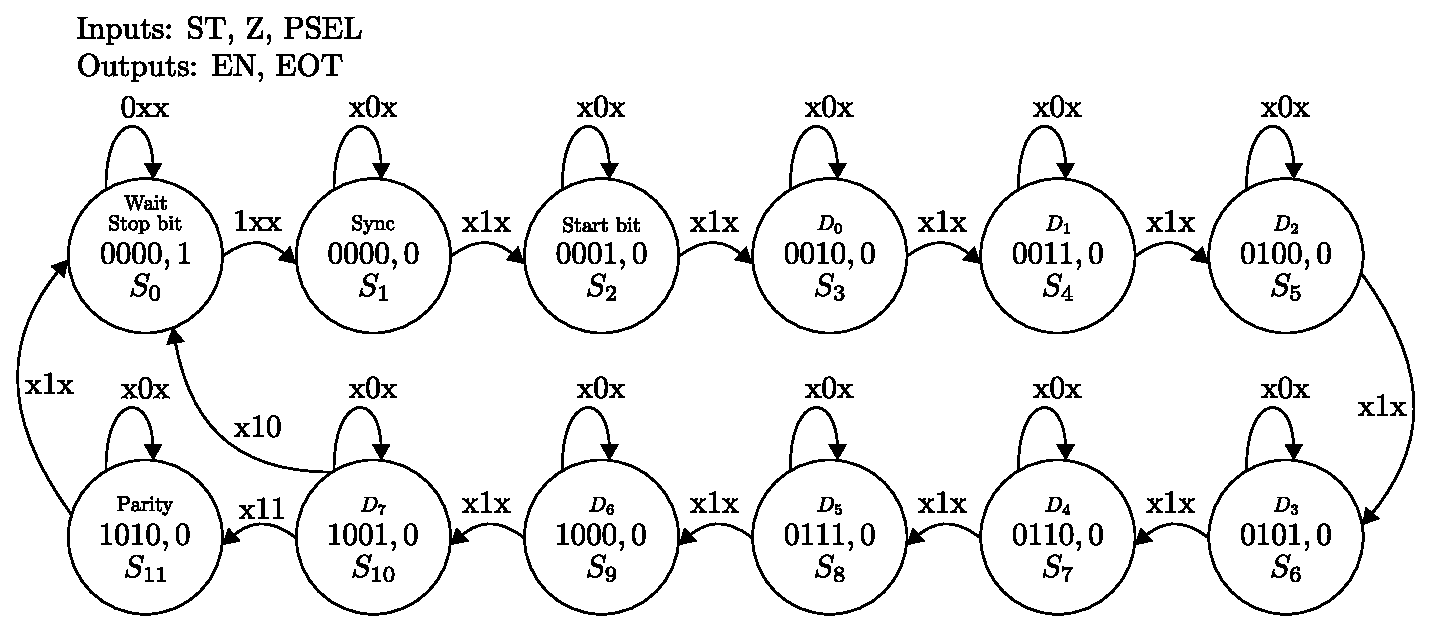
\includegraphics[width=0.8\linewidth]{C0_fsm_rs232}
		\label{fig:C0_fsm_rs232}
	\end{figure}	
	
	
	\begin{figure}[hbtp]
		\caption{Arquitectura de transmisión.}
		\centering
		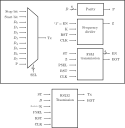
\includegraphics[width=0.6\linewidth]{C1_architecture_rs232}
		\label{fig:C1_architecture_rs232}
	\end{figure}
	
	\begin{figure}[hbtp]
		\caption{Arquitectura de TRNG.}
		\centering
		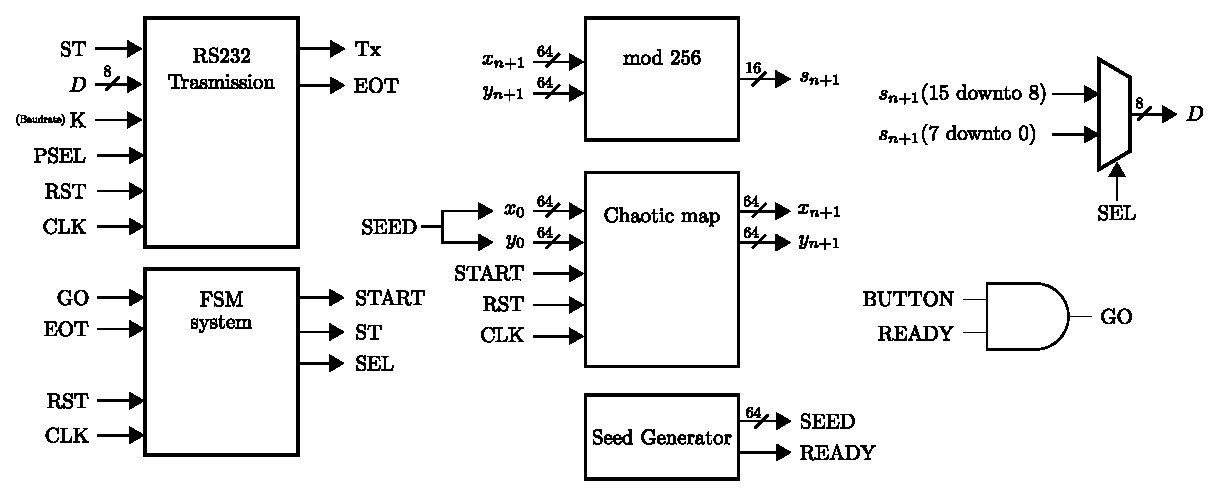
\includegraphics[width=0.9\linewidth]{D0_system}
		\label{fig:D0_system}
	\end{figure}
	
	\begin{figure}[hbtp]
		\caption{Máquina de estados de arquitectura de TRNG.}
		\centering
		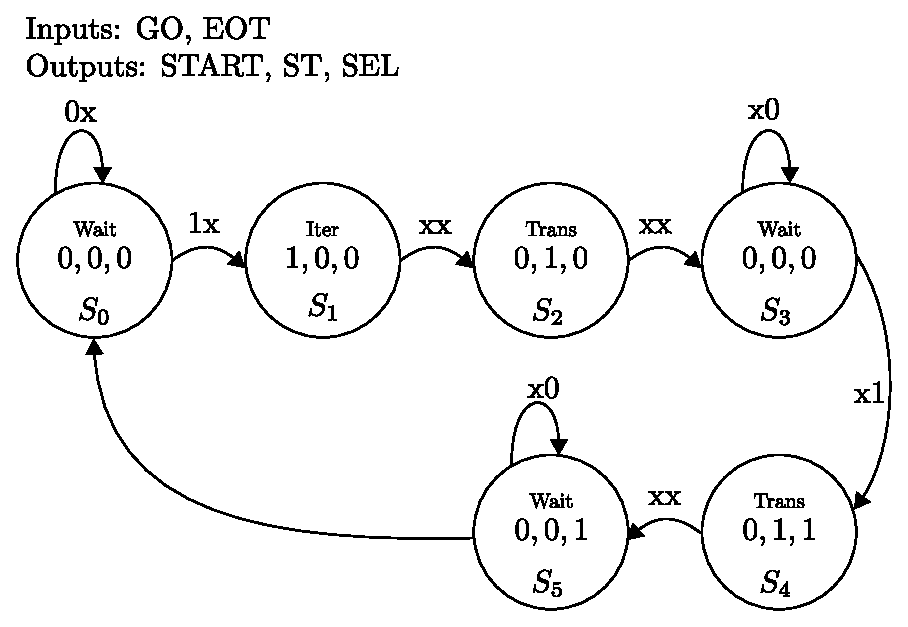
\includegraphics[width=0.7\linewidth]{D1_fsm_system}
		\label{fig:D1_fsm_system}
	\end{figure}
	

	
\begin{table}[htbp]
  \centering
  \caption{Resumen de los resultados de implementación de las TRNGs}
\resizebox{0.5\linewidth}{!}{ 
    \begin{tabular}{lll}
   & Test name                 & Prop. \\
   \hline
1  & Frequency                 & 0.99  \\
2  & Block frequency           & 0.99  \\
3  & Runs                      & 1.00     \\
4  & Longest run               & 1.0     \\
5  & Rank                      & 0.98  \\
6  & DFT                       & 0.99  \\
7  & Non-overlapping templates & 1.00     \\
8  & Overlapping templates     & 0.99  \\
9  & Universal                 & 0.99  \\
10 & Linear complexity         & 0.99  \\
11 & Serial                    & 0.99  \\
12 & Approximate Entropy       & 0.99  \\
13 & Cumulative Sums           & 0.99  \\
14 & Random excursions         & 0.99  \\
15 & Random excursions variant & 1.00    
    \end{tabular}
}
  \label{tab:asdasd}
\end{table}


\newpage
	Para poder realizar la implementación del núcleo ERO es necesario utilizar las primitivas y macros propias del fabricante de FPGA que para este trabajo es Xilinx. Las primitivas son componentes de Xilinx que son nativos de la arquitectura a la que se dirige y los macros son elementos que se encuentran en las bibliotecas UniMacro y Xilinx Parameterized Macros, las cuales se utilizan para instanciar elementos que son complejos de instanciar simplemente usando las primitivas, después las herramientas de síntesis expanden automáticamente estas macros a sus primitivas subyacentes. Los métodos de diseño disponibles son la instanciación, la inferencia, el catalogo IP y el soporte de macros, no obstante para este diseño solo se utilizan la instanciación, la cual permite instanciar un componente directamente en el diseño y es útil si se desea controlar el uso, la implementación y la ubicación exactos de los bloques individuales y el soporte de macros, el cual, utilizando las librerías antes mencionadas permiten abstraer la complejidad de utilizar unicamente primitivas simples.
	
	Toda la información referente a los macros y primitivas se encuentran en la documentación oficial en el archivo llamado ``Vivado Design Suite 7 Series FPGA Libraries Guide''. Para poder utilizar las primitivas y las macros es necesario agregar la librería UniMacro en la cabecera del archivo VHDL de la siguiente manera: 

\vspace{0.4cm}
\begin{lstlisting}[style = VHDL_TEXT]
LIBRARY UNISIM;
USE UNISIM.vcomponents.ALL;
\end{lstlisting}

	\section{Primitivas}
	
		\subsection{LUT1: 1-Bit Look-Up Table with General Output}
	
	\begin{figure}[hbtp]
		\caption{Esquemático de LUT1.}
		\centering
		\includegraphics[width=0.3\linewidth]{D3_lut1}
		\label{fig:D2_lut1}
	\end{figure}	
	
Este elemento proporciona una versión de look-up table de un búfer o inversor. Estos elementos son los bloques de construcción básicos. El parámetro INIT le da a la LUT su valor lógico. De forma predeterminada, este valor es cero, lo que lleva la salida a cero independientemente de los valores de entrada (actuando como tierra).Sin embargo, en la mayoría de los casos hay que determinar un nuevo valor INIT para especificar la función lógica de la primitiva LUT. Existen al menos dos métodos mediante los cuales se puede determinar el valor LUT. El método de la tabla lógica y el método de ecuación. En la Tabla \ref{tab:lut1} se muestran las entradas y salidas y la forma de configurar INIT y en el Código \ref{cod:lut1} se muestra su implementación en VHDL.


	\begin{table}[htbp]
		\centering
		\caption{Tabla lógica de LUT1.}
		\begin{tabular}{|cc|}
		\hline
		\multicolumn{1}{|c|}{\textbf{Inputs}} & \textbf{Outputs} \\ 
		\multicolumn{1}{|c|}{\textbf{I0}} & \textbf{O} \\ \hline 
		\multicolumn{1}{|c|}{0} & INIT[0] \\ \hline
		\multicolumn{1}{|c|}{1} & INIT[1] \\ \hline
		\multicolumn{2}{|c|}{INIT = Binary number assigned to the INIT attribute}          \\ \hline
		\end{tabular}
		\label{tab:lut1}
	\end{table}	
	

\vspace{0.4cm}
\begin{lstlisting}[style = VHDL_TEXT, caption = Primitiva LUT1., label = cod:lut1]
Library UNISIM;
use UNISIM.vcomponents.all;
-- LUT1: 1-input Look-Up Table with general output
-- 7 Series
-- Xilinx HDL Language Template, version 2021.2
LUT1_inst : LUT1
generic map (
    INIT => "00")
port map (
    O => O, -- LUT general output
    I0 => I0 -- LUT input
);
-- End of LUT1_inst instantiation
\end{lstlisting}






	\subsection{OBUFDS: Differential Signaling Output Buffer}
	
	\begin{figure}[hbtp]
		\caption{Esquemático de OBUFDS.}
		\centering
		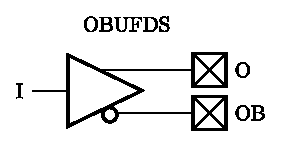
\includegraphics[width=0.3\linewidth]{D3_obufds}
		\label{fig:D3_obufds}
	\end{figure}	
	
	Este elemento de diseño es un búfer de salida única que admite señalización diferencial de bajo voltaje. OBUFDS aísla el circuito interno y proporciona corriente de accionamiento para las señales que salen del chip. Su salida se representa como dos puertos distintos (O y OB), uno considerado el ``maestro'' y el otro el ``esclavo''. El maestro y el esclavo son fases opuestas de la misma señal lógica.  En la Tabla \ref{tab:obufsd} se muestran las entradas y salidas y en el Código \ref{cod:obufsd} se muestra su implementación en VHDL.

	
	\begin{table}[htbp]
		\centering
		\caption{Tabla lógica de OBUFDS.}
		\begin{tabular}{|c|cc|}
		\hline
		\textbf{Inputs} & \multicolumn{2}{c|}{\textbf{Outputs}} \\ 
		\textbf{I}      & \multicolumn{1}{c}{\textbf{O}}  & \textbf{OB} \\ \hline
		0      & \multicolumn{1}{c|}{0}  & 1  \\ \hline
		1      & \multicolumn{1}{c|}{1}  & 0  \\ \hline
		\end{tabular}
		\label{tab:obufsd}
	\end{table}


\vspace{0.4cm}
\begin{lstlisting}[style = VHDL_TEXT, caption = Primitiva OBUFDS., label = cod:obufsd]
Library UNISIM;
use UNISIM.vcomponents.all;
-- OBUFDS: Differential Output Buffer
-- 7 Series
-- Xilinx HDL Language Template, version 2021.2
OBUFDS_inst : OBUFDS
generic map (
    IOSTANDARD => "DEFAULT", -- Specify the output I/O standard
    SLEW => "SLOW") -- Specify the output slew rate
port map (
    O => O, -- Diff_p output (connect directly to top-level port)
    OB => OB, -- Diff_n output (connect directly to top-level port)
    I => I -- Buffer input
);
-- End of OBUFDS_inst instantiation
\end{lstlisting}



Datos para programar la tarjeta

Default Board: Basys3
Default Part: xc7a35tcpg236-1
Product: Artix-7
Family: Artix-7
Package: cpg236
Speed Grade: -1








	\chapter{Conclusiones}
    Aquí van las conclusiones.
	

	Comprobación de glosarios

\Gls{FPGA} 

\Gls{RNG} 

\Gls{TRNG}

\Gls{TERO}

\Gls{ERO-TRNG}

\Gls{COSO-TRNG}

\Gls{MURO-TRNG}

\Gls{TERO-TRNG}

\Gls{PLL-TRNG}

\Gls{STR-TRNG}


\appendix
	\chapter{Códigos}

%\lstinputlisting[style = MATLAB, caption =  Nombre de abajo, label = cod:nombre1]{codigos/matlab/test_code.m}

	\section{Códigos en C}
\lstinputlisting[style = C, caption =  Comprobar el número de bytes de los tipos de dato del sistema., label = cod:A1]{codigos/c_codes/A1_check_sys_bytes.c}

\newpage
\lstinputlisting[style = C, caption =  Simulación de mapa caótico en punto flotante., label = cod:A2]{codigos/c_codes/A2_chaotic_map_float.c}

\newpage
\lstinputlisting[style = C, caption =  Simulación de mapa caótico en punto fijo., label = cod:A3]{codigos/c_codes/A3_chaotic_map_fixed.c}

\newpage
\lstinputlisting[style = C, caption = Generador de memoria ROM de condiciones iniciales., label = cod:A4]{codigos/c_codes/A4_rom_gen_chaotic_map.c}

\newpage
\lstinputlisting[style = C, caption =  Convertidor de punto flotante a punto fijo., label = cod:A5]{codigos/c_codes/A5_fixed_point_converter.c}

\newpage
\lstinputlisting[style = C, caption = Simulación de mapa caótico en punto fijo y operación mod 256., label = cod:A6]{codigos/c_codes/A6_chaotic_map_mod.c}

\newpage
\lstinputlisting[style = C, caption = Simulación de mapa caótico en punto fijo y operación mod 256 salida binaria., label = cod:A7]{codigos/c_codes/A7_chaotic_map_mod_bin.c}

    \section{Códigos en VHDL de mapa caótico}

\lstinputlisting[style = VHDL, caption = Multiplexor para control de condición inicial y retroalimentación., label = cod:mux_ic]{codigos/vhdl_codes/chaotic_map/mux_ic.vhd}

\lstinputlisting[style = VHDL, caption = Sumador genérico compatible con punto fijo., label = cod:adder]{codigos/vhdl_codes/chaotic_map/adder.vhd}

\newpage
\lstinputlisting[style = VHDL, caption = ROM para almacenar parámetros en punto fijo del mapa caótico., label = cod:rom_cm]{codigos/vhdl_codes/chaotic_map/rom_cm.vhd}

\lstinputlisting[style = VHDL, caption = Multiplicador en punto fijo con truncamiento., label = cod:mult]{codigos/vhdl_codes/chaotic_map/mult.vhd}

\lstinputlisting[style = VHDL, caption = Flip-Flop con habilitación., label = cod:ff_hab]{codigos/vhdl_codes/chaotic_map/ff_hab.vhd}

% \newpage
\lstinputlisting[style = VHDL, caption = Máquina de estados para control de las iteraciones del mapa caótico., label = cod:fsm_cm]{codigos/vhdl_codes/chaotic_map/fsm_cm.vhd}

% \newpage
\lstinputlisting[style = VHDL, caption = Descripción completa del mapa caótico., label = cod:chaotic_map]{codigos/vhdl_codes/chaotic_map/chaotic_map.vhd}


% \newpage
% 	\section{Códigos en VHDL de comunicación RS232}
% \lstinputlisting[style = VHDL, caption = Divisor de frecuencia., label = cod:freq_div]{codigos/vhdl_codes/rs232/freq_div.vhd}

% \newpage
% \lstinputlisting[style = VHDL, caption = Detector de paridad tipo par., label = cod:parity]{codigos/vhdl_codes/rs232/parity.vhd}

% \lstinputlisting[style = VHDL, caption = Multiplexor para la selección de bits de la comunicación., label = cod:mux_trans]{codigos/vhdl_codes/rs232/mux_trans.vhd}

% \newpage
% \lstinputlisting[style = VHDL, caption = Transmisión del protocolo RS232., label = cod:transmission]{codigos/vhdl_codes/rs232/transmission.vhd}

% \lstinputlisting[style = VHDL, caption = Testbench de comunicación RS232., label = cod:tb_trans]{codigos/vhdl_codes/rs232/tb_trans.vhd}

% \newpage
% \lstinputlisting[style = VHDL, caption = Máquina de estados para el control de la transmisión., label = cod:fsm_trans]{codigos/vhdl_codes/rs232/fsm_trans.vhd}

% 	\section{Códigos en VHDL de ERO}


% \newpage
% 	\section{Códigos en VHDL de arquitectura TRNG}
% \lstinputlisting[style = VHDL, caption = Multiplexor para conexión con la comunicación RS232., label = cod:mux_system_mod]{codigos/vhdl_codes/trng/mux_system_mod.vhd}

% \lstinputlisting[style = VHDL, caption = Operación mod 256., label = cod:mod_256]{codigos/vhdl_codes/trng/mod_256.vhd}

% \newpage
% \lstinputlisting[style = VHDL, caption = Máquina de estados de sistema TRNG., label = cod:fsm_system_mod]{codigos/vhdl_codes/trng/fsm_system_mod.vhd}

% \newpage
% \lstinputlisting[style = VHDL, caption = Descripción de arquitectura TRNG., label = cod:system_mod]{codigos/vhdl_codes/trng/system_mod.vhd}


\backmatter

%\nocite{*}
\bibliographystyle{ieeetr}
\bibliography{bibliografia}

\end{document}
